
% Default to the notebook output style

    


% Inherit from the specified cell style.




    
\documentclass{article}

    
    
    \usepackage{graphicx} % Used to insert images
    \usepackage{adjustbox} % Used to constrain images to a maximum size 
    \usepackage{color} % Allow colors to be defined
    \usepackage{enumerate} % Needed for markdown enumerations to work
    \usepackage{geometry} % Used to adjust the document margins
    \usepackage{amsmath} % Equations
    \usepackage{amssymb} % Equations
    \usepackage[mathletters]{ucs} % Extended unicode (utf-8) support
    \usepackage[utf8x]{inputenc} % Allow utf-8 characters in the tex document
    \usepackage{fancyvrb} % verbatim replacement that allows latex
    \usepackage{grffile} % extends the file name processing of package graphics 
                         % to support a larger range 
    % The hyperref package gives us a pdf with properly built
    % internal navigation ('pdf bookmarks' for the table of contents,
    % internal cross-reference links, web links for URLs, etc.)
    \usepackage{hyperref}
    \usepackage{longtable} % longtable support required by pandoc >1.10
    \usepackage{booktabs}  % table support for pandoc > 1.12.2
    

    
    
    \definecolor{orange}{cmyk}{0,0.4,0.8,0.2}
    \definecolor{darkorange}{rgb}{.71,0.21,0.01}
    \definecolor{darkgreen}{rgb}{.12,.54,.11}
    \definecolor{myteal}{rgb}{.26, .44, .56}
    \definecolor{gray}{gray}{0.45}
    \definecolor{lightgray}{gray}{.95}
    \definecolor{mediumgray}{gray}{.8}
    \definecolor{inputbackground}{rgb}{.95, .95, .85}
    \definecolor{outputbackground}{rgb}{.95, .95, .95}
    \definecolor{traceback}{rgb}{1, .95, .95}
    % ansi colors
    \definecolor{red}{rgb}{.6,0,0}
    \definecolor{green}{rgb}{0,.65,0}
    \definecolor{brown}{rgb}{0.6,0.6,0}
    \definecolor{blue}{rgb}{0,.145,.698}
    \definecolor{purple}{rgb}{.698,.145,.698}
    \definecolor{cyan}{rgb}{0,.698,.698}
    \definecolor{lightgray}{gray}{0.5}
    
    % bright ansi colors
    \definecolor{darkgray}{gray}{0.25}
    \definecolor{lightred}{rgb}{1.0,0.39,0.28}
    \definecolor{lightgreen}{rgb}{0.48,0.99,0.0}
    \definecolor{lightblue}{rgb}{0.53,0.81,0.92}
    \definecolor{lightpurple}{rgb}{0.87,0.63,0.87}
    \definecolor{lightcyan}{rgb}{0.5,1.0,0.83}
    
    % commands and environments needed by pandoc snippets
    % extracted from the output of `pandoc -s`
    \DefineVerbatimEnvironment{Highlighting}{Verbatim}{commandchars=\\\{\}}
    % Add ',fontsize=\small' for more characters per line
    \newenvironment{Shaded}{}{}
    \newcommand{\KeywordTok}[1]{\textcolor[rgb]{0.00,0.44,0.13}{\textbf{{#1}}}}
    \newcommand{\DataTypeTok}[1]{\textcolor[rgb]{0.56,0.13,0.00}{{#1}}}
    \newcommand{\DecValTok}[1]{\textcolor[rgb]{0.25,0.63,0.44}{{#1}}}
    \newcommand{\BaseNTok}[1]{\textcolor[rgb]{0.25,0.63,0.44}{{#1}}}
    \newcommand{\FloatTok}[1]{\textcolor[rgb]{0.25,0.63,0.44}{{#1}}}
    \newcommand{\CharTok}[1]{\textcolor[rgb]{0.25,0.44,0.63}{{#1}}}
    \newcommand{\StringTok}[1]{\textcolor[rgb]{0.25,0.44,0.63}{{#1}}}
    \newcommand{\CommentTok}[1]{\textcolor[rgb]{0.38,0.63,0.69}{\textit{{#1}}}}
    \newcommand{\OtherTok}[1]{\textcolor[rgb]{0.00,0.44,0.13}{{#1}}}
    \newcommand{\AlertTok}[1]{\textcolor[rgb]{1.00,0.00,0.00}{\textbf{{#1}}}}
    \newcommand{\FunctionTok}[1]{\textcolor[rgb]{0.02,0.16,0.49}{{#1}}}
    \newcommand{\RegionMarkerTok}[1]{{#1}}
    \newcommand{\ErrorTok}[1]{\textcolor[rgb]{1.00,0.00,0.00}{\textbf{{#1}}}}
    \newcommand{\NormalTok}[1]{{#1}}
    
    % Define a nice break command that doesn't care if a line doesn't already
    % exist.
    \def\br{\hspace*{\fill} \\* }
    % Math Jax compatability definitions
    \def\gt{>}
    \def\lt{<}
    % Document parameters
    \title{GrahamGroup}
    
    
    

    % Pygments definitions
    
\makeatletter
\def\PY@reset{\let\PY@it=\relax \let\PY@bf=\relax%
    \let\PY@ul=\relax \let\PY@tc=\relax%
    \let\PY@bc=\relax \let\PY@ff=\relax}
\def\PY@tok#1{\csname PY@tok@#1\endcsname}
\def\PY@toks#1+{\ifx\relax#1\empty\else%
    \PY@tok{#1}\expandafter\PY@toks\fi}
\def\PY@do#1{\PY@bc{\PY@tc{\PY@ul{%
    \PY@it{\PY@bf{\PY@ff{#1}}}}}}}
\def\PY#1#2{\PY@reset\PY@toks#1+\relax+\PY@do{#2}}

\expandafter\def\csname PY@tok@gd\endcsname{\def\PY@tc##1{\textcolor[rgb]{0.63,0.00,0.00}{##1}}}
\expandafter\def\csname PY@tok@gu\endcsname{\let\PY@bf=\textbf\def\PY@tc##1{\textcolor[rgb]{0.50,0.00,0.50}{##1}}}
\expandafter\def\csname PY@tok@gt\endcsname{\def\PY@tc##1{\textcolor[rgb]{0.00,0.27,0.87}{##1}}}
\expandafter\def\csname PY@tok@gs\endcsname{\let\PY@bf=\textbf}
\expandafter\def\csname PY@tok@gr\endcsname{\def\PY@tc##1{\textcolor[rgb]{1.00,0.00,0.00}{##1}}}
\expandafter\def\csname PY@tok@cm\endcsname{\let\PY@it=\textit\def\PY@tc##1{\textcolor[rgb]{0.25,0.50,0.50}{##1}}}
\expandafter\def\csname PY@tok@vg\endcsname{\def\PY@tc##1{\textcolor[rgb]{0.10,0.09,0.49}{##1}}}
\expandafter\def\csname PY@tok@m\endcsname{\def\PY@tc##1{\textcolor[rgb]{0.40,0.40,0.40}{##1}}}
\expandafter\def\csname PY@tok@mh\endcsname{\def\PY@tc##1{\textcolor[rgb]{0.40,0.40,0.40}{##1}}}
\expandafter\def\csname PY@tok@go\endcsname{\def\PY@tc##1{\textcolor[rgb]{0.53,0.53,0.53}{##1}}}
\expandafter\def\csname PY@tok@ge\endcsname{\let\PY@it=\textit}
\expandafter\def\csname PY@tok@vc\endcsname{\def\PY@tc##1{\textcolor[rgb]{0.10,0.09,0.49}{##1}}}
\expandafter\def\csname PY@tok@il\endcsname{\def\PY@tc##1{\textcolor[rgb]{0.40,0.40,0.40}{##1}}}
\expandafter\def\csname PY@tok@cs\endcsname{\let\PY@it=\textit\def\PY@tc##1{\textcolor[rgb]{0.25,0.50,0.50}{##1}}}
\expandafter\def\csname PY@tok@cp\endcsname{\def\PY@tc##1{\textcolor[rgb]{0.74,0.48,0.00}{##1}}}
\expandafter\def\csname PY@tok@gi\endcsname{\def\PY@tc##1{\textcolor[rgb]{0.00,0.63,0.00}{##1}}}
\expandafter\def\csname PY@tok@gh\endcsname{\let\PY@bf=\textbf\def\PY@tc##1{\textcolor[rgb]{0.00,0.00,0.50}{##1}}}
\expandafter\def\csname PY@tok@ni\endcsname{\let\PY@bf=\textbf\def\PY@tc##1{\textcolor[rgb]{0.60,0.60,0.60}{##1}}}
\expandafter\def\csname PY@tok@nl\endcsname{\def\PY@tc##1{\textcolor[rgb]{0.63,0.63,0.00}{##1}}}
\expandafter\def\csname PY@tok@nn\endcsname{\let\PY@bf=\textbf\def\PY@tc##1{\textcolor[rgb]{0.00,0.00,1.00}{##1}}}
\expandafter\def\csname PY@tok@no\endcsname{\def\PY@tc##1{\textcolor[rgb]{0.53,0.00,0.00}{##1}}}
\expandafter\def\csname PY@tok@na\endcsname{\def\PY@tc##1{\textcolor[rgb]{0.49,0.56,0.16}{##1}}}
\expandafter\def\csname PY@tok@nb\endcsname{\def\PY@tc##1{\textcolor[rgb]{0.00,0.50,0.00}{##1}}}
\expandafter\def\csname PY@tok@nc\endcsname{\let\PY@bf=\textbf\def\PY@tc##1{\textcolor[rgb]{0.00,0.00,1.00}{##1}}}
\expandafter\def\csname PY@tok@nd\endcsname{\def\PY@tc##1{\textcolor[rgb]{0.67,0.13,1.00}{##1}}}
\expandafter\def\csname PY@tok@ne\endcsname{\let\PY@bf=\textbf\def\PY@tc##1{\textcolor[rgb]{0.82,0.25,0.23}{##1}}}
\expandafter\def\csname PY@tok@nf\endcsname{\def\PY@tc##1{\textcolor[rgb]{0.00,0.00,1.00}{##1}}}
\expandafter\def\csname PY@tok@si\endcsname{\let\PY@bf=\textbf\def\PY@tc##1{\textcolor[rgb]{0.73,0.40,0.53}{##1}}}
\expandafter\def\csname PY@tok@s2\endcsname{\def\PY@tc##1{\textcolor[rgb]{0.73,0.13,0.13}{##1}}}
\expandafter\def\csname PY@tok@vi\endcsname{\def\PY@tc##1{\textcolor[rgb]{0.10,0.09,0.49}{##1}}}
\expandafter\def\csname PY@tok@nt\endcsname{\let\PY@bf=\textbf\def\PY@tc##1{\textcolor[rgb]{0.00,0.50,0.00}{##1}}}
\expandafter\def\csname PY@tok@nv\endcsname{\def\PY@tc##1{\textcolor[rgb]{0.10,0.09,0.49}{##1}}}
\expandafter\def\csname PY@tok@s1\endcsname{\def\PY@tc##1{\textcolor[rgb]{0.73,0.13,0.13}{##1}}}
\expandafter\def\csname PY@tok@sh\endcsname{\def\PY@tc##1{\textcolor[rgb]{0.73,0.13,0.13}{##1}}}
\expandafter\def\csname PY@tok@sc\endcsname{\def\PY@tc##1{\textcolor[rgb]{0.73,0.13,0.13}{##1}}}
\expandafter\def\csname PY@tok@sx\endcsname{\def\PY@tc##1{\textcolor[rgb]{0.00,0.50,0.00}{##1}}}
\expandafter\def\csname PY@tok@bp\endcsname{\def\PY@tc##1{\textcolor[rgb]{0.00,0.50,0.00}{##1}}}
\expandafter\def\csname PY@tok@c1\endcsname{\let\PY@it=\textit\def\PY@tc##1{\textcolor[rgb]{0.25,0.50,0.50}{##1}}}
\expandafter\def\csname PY@tok@kc\endcsname{\let\PY@bf=\textbf\def\PY@tc##1{\textcolor[rgb]{0.00,0.50,0.00}{##1}}}
\expandafter\def\csname PY@tok@c\endcsname{\let\PY@it=\textit\def\PY@tc##1{\textcolor[rgb]{0.25,0.50,0.50}{##1}}}
\expandafter\def\csname PY@tok@mf\endcsname{\def\PY@tc##1{\textcolor[rgb]{0.40,0.40,0.40}{##1}}}
\expandafter\def\csname PY@tok@err\endcsname{\def\PY@bc##1{\setlength{\fboxsep}{0pt}\fcolorbox[rgb]{1.00,0.00,0.00}{1,1,1}{\strut ##1}}}
\expandafter\def\csname PY@tok@kd\endcsname{\let\PY@bf=\textbf\def\PY@tc##1{\textcolor[rgb]{0.00,0.50,0.00}{##1}}}
\expandafter\def\csname PY@tok@ss\endcsname{\def\PY@tc##1{\textcolor[rgb]{0.10,0.09,0.49}{##1}}}
\expandafter\def\csname PY@tok@sr\endcsname{\def\PY@tc##1{\textcolor[rgb]{0.73,0.40,0.53}{##1}}}
\expandafter\def\csname PY@tok@mo\endcsname{\def\PY@tc##1{\textcolor[rgb]{0.40,0.40,0.40}{##1}}}
\expandafter\def\csname PY@tok@kn\endcsname{\let\PY@bf=\textbf\def\PY@tc##1{\textcolor[rgb]{0.00,0.50,0.00}{##1}}}
\expandafter\def\csname PY@tok@mi\endcsname{\def\PY@tc##1{\textcolor[rgb]{0.40,0.40,0.40}{##1}}}
\expandafter\def\csname PY@tok@gp\endcsname{\let\PY@bf=\textbf\def\PY@tc##1{\textcolor[rgb]{0.00,0.00,0.50}{##1}}}
\expandafter\def\csname PY@tok@o\endcsname{\def\PY@tc##1{\textcolor[rgb]{0.40,0.40,0.40}{##1}}}
\expandafter\def\csname PY@tok@kr\endcsname{\let\PY@bf=\textbf\def\PY@tc##1{\textcolor[rgb]{0.00,0.50,0.00}{##1}}}
\expandafter\def\csname PY@tok@s\endcsname{\def\PY@tc##1{\textcolor[rgb]{0.73,0.13,0.13}{##1}}}
\expandafter\def\csname PY@tok@kp\endcsname{\def\PY@tc##1{\textcolor[rgb]{0.00,0.50,0.00}{##1}}}
\expandafter\def\csname PY@tok@w\endcsname{\def\PY@tc##1{\textcolor[rgb]{0.73,0.73,0.73}{##1}}}
\expandafter\def\csname PY@tok@kt\endcsname{\def\PY@tc##1{\textcolor[rgb]{0.69,0.00,0.25}{##1}}}
\expandafter\def\csname PY@tok@ow\endcsname{\let\PY@bf=\textbf\def\PY@tc##1{\textcolor[rgb]{0.67,0.13,1.00}{##1}}}
\expandafter\def\csname PY@tok@sb\endcsname{\def\PY@tc##1{\textcolor[rgb]{0.73,0.13,0.13}{##1}}}
\expandafter\def\csname PY@tok@k\endcsname{\let\PY@bf=\textbf\def\PY@tc##1{\textcolor[rgb]{0.00,0.50,0.00}{##1}}}
\expandafter\def\csname PY@tok@se\endcsname{\let\PY@bf=\textbf\def\PY@tc##1{\textcolor[rgb]{0.73,0.40,0.13}{##1}}}
\expandafter\def\csname PY@tok@sd\endcsname{\let\PY@it=\textit\def\PY@tc##1{\textcolor[rgb]{0.73,0.13,0.13}{##1}}}

\def\PYZbs{\char`\\}
\def\PYZus{\char`\_}
\def\PYZob{\char`\{}
\def\PYZcb{\char`\}}
\def\PYZca{\char`\^}
\def\PYZam{\char`\&}
\def\PYZlt{\char`\<}
\def\PYZgt{\char`\>}
\def\PYZsh{\char`\#}
\def\PYZpc{\char`\%}
\def\PYZdl{\char`\$}
\def\PYZhy{\char`\-}
\def\PYZsq{\char`\'}
\def\PYZdq{\char`\"}
\def\PYZti{\char`\~}
% for compatibility with earlier versions
\def\PYZat{@}
\def\PYZlb{[}
\def\PYZrb{]}
\makeatother


    % Exact colors from NB
    \definecolor{incolor}{rgb}{0.0, 0.0, 0.5}
    \definecolor{outcolor}{rgb}{0.545, 0.0, 0.0}



    
    % Prevent overflowing lines due to hard-to-break entities
    \sloppy 
    % Setup hyperref package
    \hypersetup{
      breaklinks=true,  % so long urls are correctly broken across lines
      colorlinks=true,
      urlcolor=blue,
      linkcolor=darkorange,
      citecolor=darkgreen,
      }
    % Slightly bigger margins than the latex defaults
    
    \geometry{verbose,tmargin=1in,bmargin=1in,lmargin=1in,rmargin=1in}
    
    

    \begin{document}
    
    
    \maketitle
    
    

    

    \section{Robust Extraction of Quantitative Information from Histology Images}



    \paragraph{Quentin Caudron Romain Garnier \emph{with Bryan Grenfell and Andrea
Graham}}



    \subsubsection{Outline}


    \begin{itemize}
\itemsep1pt\parskip0pt\parsep0pt
\item
  Image processing
\item
  Extracted measures
\item
  Preliminary analysis
\item
  Future directions
\end{itemize}

    \begin{enumerate}
\def\labelenumi{\arabic{enumi}.}
\setcounter{enumi}{3}
\itemsep1pt\parskip0pt\parsep0pt
\item
  Age as random effect \textless{}---
\end{enumerate}

{[}``interface\_hepatitis'', ``confluent\_necrosis'',
``portal\_inflammation'', ``ln\_ap\_ri''{]}

    \begin{Verbatim}[commandchars=\\\{\}]
{\color{incolor}In [{\color{incolor}3}]:} \PY{k}{def} \PY{n+nf}{normalise}\PY{p}{(}\PY{n}{df}\PY{p}{,} \PY{n}{skip} \PY{o}{=} \PY{p}{[}\PY{p}{]}\PY{p}{)} \PY{p}{:}
        	\PY{k}{for} \PY{n}{i} \PY{o+ow}{in} \PY{n}{df}\PY{o}{.}\PY{n}{columns} \PY{p}{:}
        		\PY{k}{if} \PY{n}{i} \PY{o+ow}{not} \PY{o+ow}{in} \PY{n}{skip} \PY{p}{:}
        			\PY{n}{df}\PY{p}{[}\PY{n}{i}\PY{p}{]} \PY{o}{\PYZhy{}}\PY{o}{=} \PY{n}{df}\PY{p}{[}\PY{n}{i}\PY{p}{]}\PY{o}{.}\PY{n}{mean}\PY{p}{(}\PY{p}{)}
        			\PY{n}{df}\PY{p}{[}\PY{n}{i}\PY{p}{]} \PY{o}{/}\PY{o}{=} \PY{n}{df}\PY{p}{[}\PY{n}{i}\PY{p}{]}\PY{o}{.}\PY{n}{std}\PY{p}{(}\PY{p}{)}
        	\PY{k}{return} \PY{n}{df}
        
        
        
        
        
        
        \PY{k}{def} \PY{n+nf}{rescale}\PY{p}{(}\PY{n}{df}\PY{p}{,} \PY{n}{skip} \PY{o}{=} \PY{p}{[}\PY{p}{]}\PY{p}{)} \PY{p}{:}
            \PY{k}{for} \PY{n}{i} \PY{o+ow}{in} \PY{n}{df}\PY{o}{.}\PY{n}{columns} \PY{p}{:}
                \PY{k}{if} \PY{n}{i} \PY{o+ow}{not} \PY{o+ow}{in} \PY{n}{skip} \PY{p}{:}
                    \PY{n}{df}\PY{p}{[}\PY{n}{i}\PY{p}{]} \PY{o}{\PYZhy{}}\PY{o}{=} \PY{n}{df}\PY{p}{[}\PY{n}{i}\PY{p}{]}\PY{o}{.}\PY{n}{min}\PY{p}{(}\PY{p}{)}
                    \PY{n}{df}\PY{p}{[}\PY{n}{i}\PY{p}{]} \PY{o}{/}\PY{o}{=} \PY{n}{df}\PY{p}{[}\PY{n}{i}\PY{p}{]}\PY{o}{.}\PY{n}{max}\PY{p}{(}\PY{p}{)}
            \PY{k}{return} \PY{n}{df}
        
        
        
        \PY{c}{\PYZsh{} Remove a layer from a list}
        \PY{k}{def} \PY{n+nf}{delayer}\PY{p}{(}\PY{n}{m}\PY{p}{)} \PY{p}{:}
        	\PY{n}{out} \PY{o}{=} \PY{p}{[}\PY{p}{]}
        	\PY{k}{for} \PY{n}{i} \PY{o+ow}{in} \PY{n}{m} \PY{p}{:}
        		\PY{k}{if} \PY{n+nb}{isinstance}\PY{p}{(}\PY{n}{i}\PY{p}{,} \PY{n+nb}{list}\PY{p}{)} \PY{p}{:}
        			\PY{k}{for} \PY{n}{j} \PY{o+ow}{in} \PY{n}{i} \PY{p}{:}
        				\PY{n}{out}\PY{o}{.}\PY{n}{append}\PY{p}{(}\PY{n}{j}\PY{p}{)}
        		\PY{k}{else} \PY{p}{:}
        			\PY{n}{out}\PY{o}{.}\PY{n}{append}\PY{p}{(}\PY{n}{i}\PY{p}{)}
        	\PY{k}{return} \PY{n}{out}
        
        
        
        
        
        
        
        \PY{c}{\PYZsh{} Remove all layers from a list}
        \PY{k}{def} \PY{n+nf}{flatten}\PY{p}{(}\PY{n}{m}\PY{p}{)} \PY{p}{:}
        	\PY{n}{out} \PY{o}{=} \PY{n}{m}\PY{p}{[}\PY{p}{:}\PY{p}{]}
        
        	\PY{k}{while} \PY{n}{out} \PY{o}{!=} \PY{n}{delayer}\PY{p}{(}\PY{n}{out}\PY{p}{)} \PY{p}{:}
        		\PY{n}{out} \PY{o}{=} \PY{n}{delayer}\PY{p}{(}\PY{n}{out}\PY{p}{)}
        
        	\PY{k}{return} \PY{n}{out}
        
        
        
        
        
        
        
        
        \PY{c}{\PYZsh{} Generate all combinations of objects in a list}
        \PY{k}{def} \PY{n+nf}{combinatorial}\PY{p}{(}\PY{n}{l}\PY{p}{)} \PY{p}{:}
        	\PY{n}{out} \PY{o}{=} \PY{p}{[}\PY{p}{]}
        
        	\PY{k}{for} \PY{n}{numel} \PY{o+ow}{in} \PY{n+nb}{range}\PY{p}{(}\PY{n+nb}{len}\PY{p}{(}\PY{n}{l}\PY{p}{)}\PY{p}{)} \PY{p}{:}
        		\PY{k}{for} \PY{n}{i} \PY{o+ow}{in} \PY{n}{itertools}\PY{o}{.}\PY{n}{combinations}\PY{p}{(}\PY{n}{l}\PY{p}{,} \PY{n}{numel}\PY{o}{+}\PY{l+m+mi}{1}\PY{p}{)} \PY{p}{:}
        			\PY{n}{out}\PY{o}{.}\PY{n}{append}\PY{p}{(}\PY{n+nb}{list}\PY{p}{(}\PY{n}{i}\PY{p}{)}\PY{p}{)}
        
        	\PY{k}{return} \PY{n}{out}
        
        
        
        
        
        
        
        
        
        
        \PY{k}{def} \PY{n+nf}{pcaplot}\PY{p}{(}\PY{n}{df}\PY{p}{)} \PY{p}{:}
        
        	\PY{c}{\PYZsh{} PCA}
        	\PY{n}{pca} \PY{o}{=} \PY{n}{decomposition}\PY{o}{.}\PY{n}{PCA}\PY{p}{(}\PY{n}{whiten} \PY{o}{=} \PY{n+nb+bp}{True}\PY{p}{)}
        	\PY{n}{pca}\PY{o}{.}\PY{n}{fit}\PY{p}{(}\PY{n}{df}\PY{p}{)}
        	\PY{n}{p1} \PY{o}{=} \PY{n}{pca}\PY{o}{.}\PY{n}{components\PYZus{}}\PY{p}{[}\PY{l+m+mi}{0}\PY{p}{]} \PY{o}{/} \PY{n}{np}\PY{o}{.}\PY{n}{abs}\PY{p}{(}\PY{n}{pca}\PY{o}{.}\PY{n}{components\PYZus{}}\PY{p}{[}\PY{l+m+mi}{0}\PY{p}{]}\PY{p}{)}\PY{o}{.}\PY{n}{max}\PY{p}{(}\PY{p}{)} \PY{o}{*} \PY{n}{np}\PY{o}{.}\PY{n}{sqrt}\PY{p}{(}\PY{l+m+mi}{2}\PY{p}{)}\PY{o}{/}\PY{l+m+mi}{2}
        	\PY{n}{p2} \PY{o}{=} \PY{n}{pca}\PY{o}{.}\PY{n}{components\PYZus{}}\PY{p}{[}\PY{l+m+mi}{1}\PY{p}{]} \PY{o}{/} \PY{n}{np}\PY{o}{.}\PY{n}{abs}\PY{p}{(}\PY{n}{pca}\PY{o}{.}\PY{n}{components\PYZus{}}\PY{p}{[}\PY{l+m+mi}{1}\PY{p}{]}\PY{p}{)}\PY{o}{.}\PY{n}{max}\PY{p}{(}\PY{p}{)} \PY{o}{*} \PY{n}{np}\PY{o}{.}\PY{n}{sqrt}\PY{p}{(}\PY{l+m+mi}{2}\PY{p}{)}\PY{o}{/}\PY{l+m+mi}{2}
        
        	\PY{c}{\PYZsh{} Normalise}
        	\PY{n}{norms} \PY{o}{=} \PY{n}{np}\PY{o}{.}\PY{n}{max}\PY{p}{(}\PY{p}{[}\PY{n}{np}\PY{o}{.}\PY{n}{sqrt}\PY{p}{(}\PY{p}{(}\PY{n}{np}\PY{o}{.}\PY{n}{array}\PY{p}{(}\PY{n+nb}{zip}\PY{p}{(}\PY{n}{p1}\PY{p}{,} \PY{n}{p2}\PY{p}{)}\PY{p}{[}\PY{n}{i}\PY{p}{]}\PY{p}{)}\PY{o}{*}\PY{o}{*}\PY{l+m+mi}{2}\PY{p}{)}\PY{o}{.}\PY{n}{sum}\PY{p}{(}\PY{p}{)}\PY{p}{)} \PY{k}{for} \PY{n}{i} \PY{o+ow}{in} \PY{n+nb}{range}\PY{p}{(}\PY{n+nb}{len}\PY{p}{(}\PY{n}{p1}\PY{p}{)}\PY{p}{)}\PY{p}{]}\PY{p}{)}
        	\PY{n}{c} \PY{o}{=} \PY{n}{plt}\PY{o}{.}\PY{n}{Circle}\PY{p}{(} \PY{p}{(}\PY{l+m+mi}{0}\PY{p}{,} \PY{l+m+mi}{0}\PY{p}{)}\PY{p}{,} \PY{n}{radius} \PY{o}{=} \PY{l+m+mi}{1}\PY{p}{,} \PY{n}{alpha} \PY{o}{=} \PY{l+m+mf}{0.2}\PY{p}{)}
        	\PY{n}{plt}\PY{o}{.}\PY{n}{axes}\PY{p}{(}\PY{n}{aspect} \PY{o}{=} \PY{l+m+mi}{1}\PY{p}{)}
        	\PY{n}{plt}\PY{o}{.}\PY{n}{gca}\PY{p}{(}\PY{p}{)}\PY{o}{.}\PY{n}{add\PYZus{}artist}\PY{p}{(}\PY{n}{c}\PY{p}{)}
        
        	\PY{n}{plt}\PY{o}{.}\PY{n}{scatter}\PY{p}{(}\PY{n}{p1} \PY{o}{/} \PY{n}{norms}\PY{p}{,} \PY{n}{p2} \PY{o}{/} \PY{n}{norms}\PY{p}{)}
        	\PY{n}{plt}\PY{o}{.}\PY{n}{xlim}\PY{p}{(}\PY{p}{[}\PY{o}{\PYZhy{}}\PY{l+m+mi}{1}\PY{p}{,} \PY{l+m+mi}{1}\PY{p}{]}\PY{p}{)}
        	\PY{n}{plt}\PY{o}{.}\PY{n}{ylim}\PY{p}{(}\PY{p}{[}\PY{o}{\PYZhy{}}\PY{l+m+mi}{1}\PY{p}{,} \PY{l+m+mi}{1}\PY{p}{]}\PY{p}{)}
        
        	\PY{k}{for} \PY{n}{i}\PY{p}{,} \PY{n}{text} \PY{o+ow}{in} \PY{n+nb}{enumerate}\PY{p}{(}\PY{n}{df}\PY{o}{.}\PY{n}{columns}\PY{p}{)} \PY{p}{:}
        		\PY{n}{plt}\PY{o}{.}\PY{n}{annotate}\PY{p}{(}\PY{n}{text}\PY{p}{,} \PY{n}{xy} \PY{o}{=} \PY{p}{[}\PY{n}{p1}\PY{p}{[}\PY{n}{i}\PY{p}{]}\PY{p}{,} \PY{n}{p2}\PY{p}{[}\PY{n}{i}\PY{p}{]}\PY{p}{]}\PY{p}{)}
        
        	\PY{n}{plt}\PY{o}{.}\PY{n}{tight\PYZus{}layout}\PY{p}{(}\PY{p}{)}
        
        
        
        
        
        
        
        
        
        
        
        \PY{k}{def} \PY{n+nf}{test\PYZus{}all\PYZus{}linear}\PY{p}{(}\PY{n}{df}\PY{p}{,} \PY{n}{y}\PY{p}{,} \PY{n}{x}\PY{p}{,} \PY{n}{return\PYZus{}significant} \PY{o}{=} \PY{n+nb+bp}{False}\PY{p}{,} \PY{n}{group} \PY{o}{=} \PY{n+nb+bp}{None}\PY{p}{)} \PY{p}{:}
        
            \PY{c}{\PYZsh{} All possible combinations of independent variables}
        	\PY{n}{independent} \PY{o}{=} \PY{n}{combinatorial}\PY{p}{(}\PY{n}{x}\PY{p}{)}
        
        	\PY{n}{fits} \PY{o}{=} \PY{p}{\PYZob{}}\PY{p}{\PYZcb{}}
        	\PY{n}{pval} \PY{o}{=} \PY{p}{\PYZob{}}\PY{p}{\PYZcb{}}
        	\PY{n}{linmodels} \PY{o}{=} \PY{p}{\PYZob{}}\PY{p}{\PYZcb{}}
        	\PY{n}{qsum} \PY{o}{=} \PY{p}{\PYZob{}}\PY{p}{\PYZcb{}}
        	\PY{n}{aic} \PY{o}{=} \PY{p}{\PYZob{}}\PY{p}{\PYZcb{}}
        
        	\PY{c}{\PYZsh{} For all dependent variables, one at a time}
        	\PY{k}{for} \PY{n}{dependent} \PY{o+ow}{in} \PY{n}{y} \PY{p}{:}
        
        		\PY{k}{print} \PY{l+s}{\PYZdq{}}\PY{l+s}{Fitting for }\PY{l+s+si}{\PYZpc{}s}\PY{l+s}{.}\PY{l+s}{\PYZdq{}} \PY{o}{\PYZpc{}} \PY{n}{dependent}
        
        		\PY{c}{\PYZsh{} For all combinations of independent variables}
        		\PY{k}{for} \PY{n}{covariate} \PY{o+ow}{in} \PY{n}{independent} \PY{p}{:}
        
        			\PY{c}{\PYZsh{} Standard mixed model}
        			\PY{k}{if} \PY{n}{group} \PY{o+ow}{is} \PY{n+nb+bp}{None} \PY{p}{:}
        
        				\PY{c}{\PYZsh{} Fit a linear model}
        				\PY{n}{subset} \PY{o}{=} \PY{n}{delayer}\PY{p}{(}\PY{p}{[}\PY{n}{covariate}\PY{p}{,} \PY{n}{dependent}\PY{p}{]}\PY{p}{)}
        				\PY{n}{df2} \PY{o}{=} \PY{n}{df}\PY{p}{[}\PY{n}{delayer}\PY{p}{(}\PY{n}{subset}\PY{p}{)}\PY{p}{]}\PY{o}{.}\PY{n}{dropna}\PY{p}{(}\PY{p}{)}
        				\PY{n}{df2}\PY{p}{[}\PY{l+s}{\PYZdq{}}\PY{l+s}{Intercept}\PY{l+s}{\PYZdq{}}\PY{p}{]} \PY{o}{=} \PY{n}{np}\PY{o}{.}\PY{n}{ones}\PY{p}{(}\PY{n+nb}{len}\PY{p}{(}\PY{n}{df2}\PY{p}{)}\PY{p}{)}
                        
        				\PY{n}{ols} \PY{o}{=} \PY{n}{sm}\PY{o}{.}\PY{n}{GLS}\PY{p}{(}\PY{n}{endog} \PY{o}{=} \PY{n}{df2}\PY{p}{[}\PY{n}{dependent}\PY{p}{]}\PY{p}{,} \PY{n}{exog} \PY{o}{=} \PY{n}{df2}\PY{p}{[}\PY{n}{delayer}\PY{p}{(}\PY{p}{[}\PY{n}{covariate}\PY{p}{,} \PY{l+s}{\PYZdq{}}\PY{l+s}{Intercept}\PY{l+s}{\PYZdq{}}\PY{p}{]}\PY{p}{)}\PY{p}{]}\PY{p}{)}\PY{o}{.}\PY{n}{fit}\PY{p}{(}\PY{p}{)}
        
        				\PY{c}{\PYZsh{} Save the results}
        				\PY{k}{if} \PY{p}{(}\PY{n}{return\PYZus{}significant} \PY{o+ow}{and} \PY{n}{ols}\PY{o}{.}\PY{n}{f\PYZus{}pvalue} \PY{o}{\PYZlt{}} \PY{l+m+mf}{0.05}\PY{p}{)} \PY{o+ow}{or} \PY{p}{(}\PY{o+ow}{not} \PY{n}{return\PYZus{}significant}\PY{p}{)} \PY{p}{:}
        					\PY{n}{linmodels}\PY{o}{.}\PY{n}{setdefault}\PY{p}{(}\PY{n}{dependent}\PY{p}{,} \PY{p}{[}\PY{p}{]}\PY{p}{)}\PY{o}{.}\PY{n}{append}\PY{p}{(}\PY{n}{ols}\PY{p}{)}
        					\PY{n}{fits}\PY{o}{.}\PY{n}{setdefault}\PY{p}{(}\PY{n}{dependent}\PY{p}{,} \PY{p}{[}\PY{p}{]}\PY{p}{)}\PY{o}{.}\PY{n}{append}\PY{p}{(}\PY{n}{ols}\PY{o}{.}\PY{n}{rsquared}\PY{p}{)}
        					\PY{n}{pval}\PY{o}{.}\PY{n}{setdefault}\PY{p}{(}\PY{n}{dependent}\PY{p}{,} \PY{p}{[}\PY{p}{]}\PY{p}{)}\PY{o}{.}\PY{n}{append}\PY{p}{(}\PY{n}{ols}\PY{o}{.}\PY{n}{f\PYZus{}pvalue}\PY{p}{)}
        					\PY{n}{aic}\PY{o}{.}\PY{n}{setdefault}\PY{p}{(}\PY{n}{dependent}\PY{p}{,} \PY{p}{[}\PY{p}{]}\PY{p}{)}\PY{o}{.}\PY{n}{append}\PY{p}{(}\PY{n}{ols}\PY{o}{.}\PY{n}{aic}\PY{p}{)}
        
        
        			\PY{c}{\PYZsh{} Mixed effects model}
        			\PY{k}{else} \PY{p}{:}
        				\PY{n}{subset} \PY{o}{=} \PY{n}{delayer}\PY{p}{(}\PY{p}{[}\PY{n}{covariate}\PY{p}{,} \PY{n}{dependent}\PY{p}{,} \PY{n}{group}\PY{p}{]}\PY{p}{)}
        				\PY{n}{df2} \PY{o}{=} \PY{n}{df}\PY{p}{[}\PY{n}{delayer}\PY{p}{(}\PY{n}{subset}\PY{p}{)}\PY{p}{]}\PY{o}{.}\PY{n}{dropna}\PY{p}{(}\PY{p}{)}
        
        				\PY{c}{\PYZsh{} Fit a mixed effects model}
        				\PY{n}{ols} \PY{o}{=} \PY{n}{MixedLM}\PY{p}{(}\PY{n}{endog} \PY{o}{=} \PY{n}{df2}\PY{p}{[}\PY{n}{dependent}\PY{p}{]}\PY{p}{,} \PY{n}{exog} \PY{o}{=} \PY{n}{df2}\PY{p}{[}\PY{n}{covariate}\PY{p}{]}\PY{p}{,} \PY{n}{groups} \PY{o}{=} \PY{n}{df2}\PY{p}{[}\PY{n}{group}\PY{p}{]}\PY{p}{)}\PY{o}{.}\PY{n}{fit}\PY{p}{(}\PY{p}{)}
        
        				\PY{c}{\PYZsh{} Calculate AIC}
        				\PY{n}{linmodels}\PY{o}{.}\PY{n}{setdefault}\PY{p}{(}\PY{n}{dependent}\PY{p}{,} \PY{p}{[}\PY{p}{]}\PY{p}{)}\PY{o}{.}\PY{n}{append}\PY{p}{(}\PY{n}{ols}\PY{p}{)}
        				\PY{n}{fits}\PY{o}{.}\PY{n}{setdefault}\PY{p}{(}\PY{n}{dependent}\PY{p}{,} \PY{p}{[}\PY{p}{]}\PY{p}{)}\PY{o}{.}\PY{n}{append}\PY{p}{(}\PY{l+m+mi}{2} \PY{o}{*} \PY{p}{(}\PY{n}{ols}\PY{o}{.}\PY{n}{k\PYZus{}fe} \PY{o}{+} \PY{l+m+mi}{1}\PY{p}{)} \PY{o}{\PYZhy{}} \PY{l+m+mi}{2} \PY{o}{*} \PY{n}{ols}\PY{o}{.}\PY{n}{llf}\PY{p}{)}
        				\PY{n}{pval}\PY{o}{.}\PY{n}{setdefault}\PY{p}{(}\PY{n}{dependent}\PY{p}{,} \PY{p}{[}\PY{p}{]}\PY{p}{)}\PY{o}{.}\PY{n}{append}\PY{p}{(}\PY{n}{ols}\PY{o}{.}\PY{n}{pvalues}\PY{p}{)}
        
        	\PY{k}{if} \PY{n}{group} \PY{o+ow}{is} \PY{o+ow}{not} \PY{n+nb+bp}{None} \PY{p}{:}
        		\PY{k}{for} \PY{n}{i} \PY{o+ow}{in} \PY{n}{y} \PY{p}{:}
        			\PY{n}{f} \PY{o}{=} \PY{n}{np}\PY{o}{.}\PY{n}{array}\PY{p}{(}\PY{n}{fits}\PY{p}{[}\PY{n}{i}\PY{p}{]}\PY{p}{)}
        			\PY{n}{models} \PY{o}{=} \PY{n}{np}\PY{o}{.}\PY{n}{array}\PY{p}{(}\PY{n}{linmodels}\PY{p}{[}\PY{n}{i}\PY{p}{]}\PY{p}{)}
        			\PY{n}{idx} \PY{o}{=} \PY{n}{np}\PY{o}{.}\PY{n}{where}\PY{p}{(}\PY{n}{f} \PY{o}{\PYZhy{}} \PY{n}{f}\PY{o}{.}\PY{n}{min}\PY{p}{(}\PY{p}{)} \PY{o}{\PYZlt{}}\PY{o}{=} \PY{l+m+mi}{2}\PY{p}{)}\PY{p}{[}\PY{l+m+mi}{0}\PY{p}{]}
        			\PY{n}{bestmodelDoF} \PY{o}{=} \PY{p}{[}\PY{n}{j}\PY{o}{.}\PY{n}{k\PYZus{}fe} \PY{k}{for} \PY{n}{j} \PY{o+ow}{in} \PY{n}{np}\PY{o}{.}\PY{n}{array}\PY{p}{(}\PY{n}{linmodels}\PY{p}{[}\PY{n}{i}\PY{p}{]}\PY{p}{)}\PY{p}{[}\PY{n}{idx}\PY{p}{]}\PY{p}{]}
        			\PY{n}{bestmodels} \PY{o}{=} \PY{p}{[}\PY{n}{idx}\PY{p}{[}\PY{n}{j}\PY{p}{]} \PY{k}{for} \PY{n}{j} \PY{o+ow}{in} \PY{n}{np}\PY{o}{.}\PY{n}{where}\PY{p}{(}\PY{n}{bestmodelDoF} \PY{o}{==} \PY{n}{np}\PY{o}{.}\PY{n}{min}\PY{p}{(}\PY{n}{bestmodelDoF}\PY{p}{)}\PY{p}{)}\PY{p}{[}\PY{l+m+mi}{0}\PY{p}{]}\PY{p}{]}
        			\PY{n}{qsum}\PY{p}{[}\PY{n}{i}\PY{p}{]} \PY{o}{=} \PY{n}{models}\PY{p}{[}\PY{n}{idx}\PY{p}{[}\PY{n}{np}\PY{o}{.}\PY{n}{where}\PY{p}{(}\PY{n}{f}\PY{p}{[}\PY{n}{bestmodels}\PY{p}{]} \PY{o}{==} \PY{n}{np}\PY{o}{.}\PY{n}{min}\PY{p}{(}\PY{n}{f}\PY{p}{[}\PY{n}{bestmodels}\PY{p}{]}\PY{p}{)}\PY{p}{)}\PY{p}{]}\PY{p}{]}
        
        
        		\PY{k}{return} \PY{n}{linmodels}\PY{p}{,} \PY{n}{fits}\PY{p}{,} \PY{n}{pval}\PY{p}{,} \PY{n}{qsum}
        
        	\PY{k}{return} \PY{n}{linmodels}\PY{p}{,} \PY{n}{fits}\PY{p}{,} \PY{n}{pval}\PY{p}{,} \PY{n}{aic}
        
        	
        		
        
        
        
        
        
        
        
        
        
        
        
        
        
        
        
        \PY{k}{def} \PY{n+nf}{summary}\PY{p}{(}\PY{n}{models}\PY{p}{)} \PY{p}{:}
        
        	\PY{c}{\PYZsh{} Generate list of everything}
        	\PY{n}{r2} \PY{o}{=} \PY{n}{np}\PY{o}{.}\PY{n}{array}\PY{p}{(}\PY{p}{[}\PY{n}{m}\PY{o}{.}\PY{n}{r2} \PY{k}{for} \PY{n}{dependent} \PY{o+ow}{in} \PY{n}{models}\PY{o}{.}\PY{n}{keys}\PY{p}{(}\PY{p}{)} \PY{k}{for} \PY{n}{m} \PY{o+ow}{in} \PY{n}{models}\PY{p}{[}\PY{n}{dependent}\PY{p}{]}\PY{p}{]}\PY{p}{)}
        	\PY{n}{p} \PY{o}{=} \PY{n}{np}\PY{o}{.}\PY{n}{array}\PY{p}{(}\PY{p}{[}\PY{n}{m}\PY{o}{.}\PY{n}{f\PYZus{}stat}\PY{p}{[}\PY{l+s}{\PYZdq{}}\PY{l+s}{p\PYZhy{}value}\PY{l+s}{\PYZdq{}}\PY{p}{]} \PY{k}{for} \PY{n}{dependent} \PY{o+ow}{in} \PY{n}{models}\PY{o}{.}\PY{n}{keys}\PY{p}{(}\PY{p}{)} \PY{k}{for} \PY{n}{m} \PY{o+ow}{in} \PY{n}{models}\PY{p}{[}\PY{n}{dependent}\PY{p}{]}\PY{p}{]}\PY{p}{)}
        	\PY{n}{mod} \PY{o}{=} \PY{n}{np}\PY{o}{.}\PY{n}{array}\PY{p}{(}\PY{p}{[}\PY{n}{m} \PY{k}{for} \PY{n}{dependent} \PY{o+ow}{in} \PY{n}{models}\PY{o}{.}\PY{n}{keys}\PY{p}{(}\PY{p}{)} \PY{k}{for} \PY{n}{m} \PY{o+ow}{in} \PY{n}{models}\PY{p}{[}\PY{n}{dependent}\PY{p}{]}\PY{p}{]}\PY{p}{)}
        	\PY{n}{dependent} \PY{o}{=} \PY{n}{np}\PY{o}{.}\PY{n}{array}\PY{p}{(}\PY{p}{[}\PY{n}{dependent} \PY{k}{for} \PY{n}{dependent} \PY{o+ow}{in} \PY{n}{models}\PY{o}{.}\PY{n}{keys}\PY{p}{(}\PY{p}{)} \PY{k}{for} \PY{n}{m} \PY{o+ow}{in} \PY{n}{models}\PY{p}{[}\PY{n}{dependent}\PY{p}{]}\PY{p}{]}\PY{p}{)}
        
        	\PY{c}{\PYZsh{} Sort by R2}
        	\PY{n}{idx} \PY{o}{=} \PY{n}{np}\PY{o}{.}\PY{n}{argsort}\PY{p}{(}\PY{n}{r2}\PY{p}{)}\PY{p}{[}\PY{p}{:}\PY{p}{:}\PY{o}{\PYZhy{}}\PY{l+m+mi}{1}\PY{p}{]}
        
        	\PY{c}{\PYZsh{} Output string}
        	\PY{n}{s} \PY{o}{=} \PY{l+s}{\PYZdq{}}\PY{l+s+si}{\PYZpc{}d}\PY{l+s}{ significant regressions.}\PY{l+s+se}{\PYZbs{}n}\PY{l+s+se}{\PYZbs{}n}\PY{l+s}{\PYZdq{}} \PY{o}{\PYZpc{}} \PY{n+nb}{len}\PY{p}{(}\PY{n}{r2}\PY{p}{)}
        	\PY{n}{s} \PY{o}{+}\PY{o}{=} \PY{l+s}{\PYZdq{}}\PY{l+s}{Ten most correlated :}\PY{l+s+se}{\PYZbs{}n}\PY{l+s+se}{\PYZbs{}n}\PY{l+s}{\PYZdq{}}
        
        	\PY{c}{\PYZsh{} Print a summary of the top ten correlations}
        	\PY{k}{for} \PY{n}{i} \PY{o+ow}{in} \PY{n}{idx}\PY{p}{[}\PY{p}{:}\PY{l+m+mi}{10}\PY{p}{]} \PY{p}{:}
        		\PY{n}{s} \PY{o}{+}\PY{o}{=} \PY{p}{(}\PY{l+s}{\PYZdq{}}\PY{l+s+si}{\PYZpc{}s}\PY{l+s}{ \PYZti{} }\PY{l+s+si}{\PYZpc{}s}\PY{l+s+se}{\PYZbs{}n}\PY{l+s}{\PYZdq{}} \PY{o}{\PYZpc{}} \PY{p}{(}\PY{n}{dependent}\PY{p}{[}\PY{n}{i}\PY{p}{]}\PY{p}{,} \PY{l+s}{\PYZdq{}}\PY{l+s}{ + }\PY{l+s}{\PYZdq{}}\PY{o}{.}\PY{n}{join}\PY{p}{(}\PY{n}{mod}\PY{p}{[}\PY{n}{i}\PY{p}{]}\PY{o}{.}\PY{n}{x}\PY{o}{.}\PY{n}{columns}\PY{p}{[}\PY{p}{:}\PY{o}{\PYZhy{}}\PY{l+m+mi}{1}\PY{p}{]}\PY{p}{)}\PY{p}{)}\PY{p}{)}
        		\PY{n}{s} \PY{o}{+}\PY{o}{=} \PY{p}{(}\PY{l+s}{\PYZdq{}}\PY{l+s}{R\PYZca{}2 = }\PY{l+s+si}{\PYZpc{}f}\PY{l+s+se}{\PYZbs{}t}\PY{l+s}{p = }\PY{l+s+si}{\PYZpc{}f}\PY{l+s+se}{\PYZbs{}n}\PY{l+s+se}{\PYZbs{}n}\PY{l+s}{\PYZdq{}} \PY{o}{\PYZpc{}} \PY{p}{(}\PY{n}{r2}\PY{p}{[}\PY{n}{i}\PY{p}{]}\PY{p}{,} \PY{n}{p}\PY{p}{[}\PY{n}{i}\PY{p}{]}\PY{p}{)}\PY{p}{)}
        
        	\PY{k}{print} \PY{n}{s}
            
            
            
            
            
            
            
        \PY{k}{def} \PY{n+nf}{rstr}\PY{p}{(}\PY{n}{y}\PY{p}{,} \PY{n}{x}\PY{p}{)} \PY{p}{:}
            \PY{n}{formatstr} \PY{o}{=} \PY{l+s}{\PYZdq{}}\PY{l+s+si}{\PYZpc{}s}\PY{l+s}{ \PYZti{} }\PY{l+s}{\PYZdq{}} \PY{o}{\PYZpc{}} \PY{n}{y}
            \PY{k}{for} \PY{n}{i} \PY{o+ow}{in} \PY{n}{x}\PY{p}{[}\PY{p}{:}\PY{o}{\PYZhy{}}\PY{l+m+mi}{1}\PY{p}{]} \PY{p}{:}
                \PY{n}{formatstr} \PY{o}{+}\PY{o}{=} \PY{n+nb}{str}\PY{p}{(}\PY{n}{i}\PY{p}{)}
                \PY{n}{formatstr} \PY{o}{+}\PY{o}{=} \PY{l+s}{\PYZdq{}}\PY{l+s}{ + }\PY{l+s}{\PYZdq{}}
            \PY{n}{formatstr} \PY{o}{+}\PY{o}{=} \PY{n+nb}{str}\PY{p}{(}\PY{n}{x}\PY{p}{[}\PY{o}{\PYZhy{}}\PY{l+m+mi}{1}\PY{p}{]}\PY{p}{)}
            \PY{k}{return} \PY{n}{formatstr}
\end{Verbatim}

    \begin{Verbatim}[commandchars=\\\{\}]
{\color{incolor}In [{\color{incolor}14}]:} \PY{k+kn}{import} \PY{n+nn}{numpy} \PY{k+kn}{as} \PY{n+nn}{np}
         \PY{k+kn}{from} \PY{n+nn}{sklearn.neighbors} \PY{k+kn}{import} \PY{n}{KernelDensity}
         \PY{k+kn}{from} \PY{n+nn}{matplotlib} \PY{k+kn}{import} \PY{n}{rcParams}
         \PY{k+kn}{import} \PY{n+nn}{matplotlib.pyplot} \PY{k+kn}{as} \PY{n+nn}{plt}
         \PY{k+kn}{import} \PY{n+nn}{seaborn}
         \PY{k+kn}{import} \PY{n+nn}{pandas} \PY{k+kn}{as} \PY{n+nn}{pd}
         \PY{k+kn}{import} \PY{n+nn}{itertools}
         \PY{k+kn}{from} \PY{n+nn}{sklearn} \PY{k+kn}{import} \PY{n}{linear\PYZus{}model}\PY{p}{,} \PY{n}{ensemble}\PY{p}{,} \PY{n}{decomposition}\PY{p}{,} \PY{n}{cross\PYZus{}validation}\PY{p}{,} \PY{n}{preprocessing}
         \PY{k+kn}{from} \PY{n+nn}{statsmodels.regression.mixed\PYZus{}linear\PYZus{}model} \PY{k+kn}{import} \PY{n}{MixedLM}
         \PY{k+kn}{import} \PY{n+nn}{statsmodels.api} \PY{k+kn}{as} \PY{n+nn}{sm}
         \PY{k+kn}{from} \PY{n+nn}{statsmodels.regression.linear\PYZus{}model} \PY{k+kn}{import} \PY{n}{OLSResults}
         \PY{k+kn}{from} \PY{n+nn}{statsmodels.tools.tools} \PY{k+kn}{import} \PY{n}{add\PYZus{}constant}
         
         
         \PY{o}{\PYZpc{}}\PY{k}{matplotlib} \PY{n}{inline}
         \PY{n}{rcParams}\PY{p}{[}\PY{l+s}{\PYZdq{}}\PY{l+s}{figure.figsize}\PY{l+s}{\PYZdq{}}\PY{p}{]} \PY{o}{=} \PY{p}{(}\PY{l+m+mi}{14}\PY{p}{,} \PY{l+m+mi}{8}\PY{p}{)}
         
         
         \PY{c}{\PYZsh{} RAW DATA}
         
         \PY{n}{raw\PYZus{}physical} \PY{o}{=} \PY{n}{pd}\PY{o}{.}\PY{n}{read\PYZus{}csv}\PY{p}{(}\PY{l+s}{\PYZdq{}}\PY{l+s}{../data/physical.csv}\PY{l+s}{\PYZdq{}}\PY{p}{)}
         \PY{n}{raw\PYZus{}histo} \PY{o}{=} \PY{n}{pd}\PY{o}{.}\PY{n}{read\PYZus{}csv}\PY{p}{(}\PY{l+s}{\PYZdq{}}\PY{l+s}{../data/tawfik.csv}\PY{l+s}{\PYZdq{}}\PY{p}{)}
         \PY{n}{ent} \PY{o}{=} \PY{n}{pd}\PY{o}{.}\PY{n}{read\PYZus{}csv}\PY{p}{(}\PY{l+s}{\PYZdq{}}\PY{l+s}{../4x/results/entropy.csv}\PY{l+s}{\PYZdq{}}\PY{p}{)}\PY{o}{.}\PY{n}{drop}\PY{p}{(}\PY{p}{[}\PY{l+s}{\PYZdq{}}\PY{l+s}{Unnamed: 0}\PY{l+s}{\PYZdq{}}\PY{p}{]}\PY{p}{,} \PY{l+m+mi}{1}\PY{p}{)}
         \PY{n}{foci} \PY{o}{=} \PY{n}{pd}\PY{o}{.}\PY{n}{read\PYZus{}csv}\PY{p}{(}\PY{l+s}{\PYZdq{}}\PY{l+s}{../4x/results/foci.csv}\PY{l+s}{\PYZdq{}}\PY{p}{)}\PY{o}{.}\PY{n}{drop}\PY{p}{(}\PY{p}{[}\PY{l+s}{\PYZdq{}}\PY{l+s}{Unnamed: 0}\PY{l+s}{\PYZdq{}}\PY{p}{]}\PY{p}{,} \PY{l+m+mi}{1}\PY{p}{)}
         \PY{n}{lac} \PY{o}{=} \PY{n}{pd}\PY{o}{.}\PY{n}{read\PYZus{}csv}\PY{p}{(}\PY{l+s}{\PYZdq{}}\PY{l+s}{../4x/results/normalised\PYZus{}lacunarity.csv}\PY{l+s}{\PYZdq{}}\PY{p}{)}\PY{o}{.}\PY{n}{drop}\PY{p}{(}\PY{p}{[}\PY{l+s}{\PYZdq{}}\PY{l+s}{Unnamed: 0}\PY{l+s}{\PYZdq{}}\PY{p}{]}\PY{p}{,} \PY{l+m+mi}{1}\PY{p}{)}
         \PY{n}{gabor} \PY{o}{=} \PY{n}{pd}\PY{o}{.}\PY{n}{read\PYZus{}csv}\PY{p}{(}\PY{l+s}{\PYZdq{}}\PY{l+s}{../4x/results/gabor\PYZus{}filters.csv}\PY{l+s}{\PYZdq{}}\PY{p}{)}\PY{o}{.}\PY{n}{drop}\PY{p}{(}\PY{p}{[}\PY{l+s}{\PYZdq{}}\PY{l+s}{Unnamed: 0}\PY{l+s}{\PYZdq{}}\PY{p}{]}\PY{p}{,} \PY{l+m+mi}{1}\PY{p}{)}
         \PY{n}{ts} \PY{o}{=} \PY{n}{pd}\PY{o}{.}\PY{n}{read\PYZus{}csv}\PY{p}{(}\PY{l+s}{\PYZdq{}}\PY{l+s}{../4x/results/tissue\PYZus{}sinusoid\PYZus{}ratio.csv}\PY{l+s}{\PYZdq{}}\PY{p}{)}\PY{o}{.}\PY{n}{drop}\PY{p}{(}\PY{p}{[}\PY{l+s}{\PYZdq{}}\PY{l+s}{Unnamed: 0}\PY{l+s}{\PYZdq{}}\PY{p}{]}\PY{p}{,} \PY{l+m+mi}{1}\PY{p}{)}
         
         \PY{n}{raw\PYZus{}image} \PY{o}{=} \PY{n}{pd}\PY{o}{.}\PY{n}{merge}\PY{p}{(}\PY{n}{lac}\PY{p}{,} \PY{n}{ent}\PY{p}{,}
         	\PY{n}{on}\PY{o}{=}\PY{p}{[}\PY{l+s}{\PYZdq{}}\PY{l+s}{Sheep}\PY{l+s}{\PYZdq{}}\PY{p}{,} \PY{l+s}{\PYZdq{}}\PY{l+s}{Image}\PY{l+s}{\PYZdq{}}\PY{p}{]}\PY{p}{)}\PY{o}{.}\PY{n}{merge}\PY{p}{(}\PY{n}{foci}\PY{p}{,} 
         	\PY{n}{on}\PY{o}{=}\PY{p}{[}\PY{l+s}{\PYZdq{}}\PY{l+s}{Sheep}\PY{l+s}{\PYZdq{}}\PY{p}{,} \PY{l+s}{\PYZdq{}}\PY{l+s}{Image}\PY{l+s}{\PYZdq{}}\PY{p}{]}\PY{p}{)}\PY{o}{.}\PY{n}{merge}\PY{p}{(}\PY{n}{gabor}\PY{p}{,}
         	\PY{n}{on}\PY{o}{=}\PY{p}{[}\PY{l+s}{\PYZdq{}}\PY{l+s}{Sheep}\PY{l+s}{\PYZdq{}}\PY{p}{,} \PY{l+s}{\PYZdq{}}\PY{l+s}{Image}\PY{l+s}{\PYZdq{}}\PY{p}{]}\PY{p}{)}\PY{o}{.}\PY{n}{merge}\PY{p}{(}\PY{n}{ts}\PY{p}{,} 
             \PY{n}{on}\PY{o}{=}\PY{p}{[}\PY{l+s}{\PYZdq{}}\PY{l+s}{Sheep}\PY{l+s}{\PYZdq{}}\PY{p}{,} \PY{l+s}{\PYZdq{}}\PY{l+s}{Image}\PY{l+s}{\PYZdq{}}\PY{p}{]}\PY{p}{)}
         \PY{n}{raw\PYZus{}image}\PY{o}{.}\PY{n}{rename}\PY{p}{(}\PY{n}{columns} \PY{o}{=} \PY{p}{\PYZob{}}	\PY{l+s}{\PYZdq{}}\PY{l+s}{meanSize}\PY{l+s}{\PYZdq{}} \PY{p}{:} \PY{l+s}{\PYZdq{}}\PY{l+s}{FociSize}\PY{l+s}{\PYZdq{}}\PY{p}{,} 
         								\PY{l+s}{\PYZdq{}}\PY{l+s}{TSRatio}\PY{l+s}{\PYZdq{}} \PY{p}{:} \PY{l+s}{\PYZdq{}}\PY{l+s}{TissueToSinusoid}\PY{l+s}{\PYZdq{}}\PY{p}{,}
         								\PY{l+s}{\PYZdq{}}\PY{l+s}{Count}\PY{l+s}{\PYZdq{}} \PY{p}{:} \PY{l+s}{\PYZdq{}}\PY{l+s}{FociCount}\PY{l+s}{\PYZdq{}} \PY{p}{\PYZcb{}}\PY{p}{,} \PY{n}{inplace}\PY{o}{=}\PY{n+nb+bp}{True}\PY{p}{)}
         
         
         
         \PY{c}{\PYZsh{} CLEAN DATA}
         
         \PY{n}{physcols} \PY{o}{=} \PY{p}{[}\PY{l+s}{\PYZdq{}}\PY{l+s}{Weight}\PY{l+s}{\PYZdq{}}\PY{p}{,} \PY{l+s}{\PYZdq{}}\PY{l+s}{Sex}\PY{l+s}{\PYZdq{}}\PY{p}{,} \PY{l+s}{\PYZdq{}}\PY{l+s}{AgeAtDeath}\PY{l+s}{\PYZdq{}}\PY{p}{,} \PY{l+s}{\PYZdq{}}\PY{l+s}{Foreleg}\PY{l+s}{\PYZdq{}}\PY{p}{,} \PY{l+s}{\PYZdq{}}\PY{l+s}{Hindleg}\PY{l+s}{\PYZdq{}}\PY{p}{]}
         \PY{n}{imagecols} \PY{o}{=} \PY{p}{[}\PY{l+s}{\PYZdq{}}\PY{l+s}{Entropy}\PY{l+s}{\PYZdq{}}\PY{p}{,} \PY{l+s}{\PYZdq{}}\PY{l+s}{Lacunarity}\PY{l+s}{\PYZdq{}}\PY{p}{,} \PY{l+s}{\PYZdq{}}\PY{l+s}{Inflammation}\PY{l+s}{\PYZdq{}}\PY{p}{,} \PY{l+s}{\PYZdq{}}\PY{l+s}{Scale}\PY{l+s}{\PYZdq{}}\PY{p}{,} \PY{l+s}{\PYZdq{}}\PY{l+s}{Directionality}\PY{l+s}{\PYZdq{}}\PY{p}{,} \PY{l+s}{\PYZdq{}}\PY{l+s}{FociCount}\PY{l+s}{\PYZdq{}}\PY{p}{,} \PY{l+s}{\PYZdq{}}\PY{l+s}{FociSize}\PY{l+s}{\PYZdq{}}\PY{p}{,} \PY{l+s}{\PYZdq{}}\PY{l+s}{TissueToSinusoid}\PY{l+s}{\PYZdq{}}\PY{p}{]}
         \PY{n}{histcols} \PY{o}{=} \PY{p}{[}\PY{l+s}{\PYZdq{}}\PY{l+s}{Lobular\PYZus{}collapse}\PY{l+s}{\PYZdq{}}\PY{p}{,} \PY{l+s}{\PYZdq{}}\PY{l+s}{Interface\PYZus{}hepatitis}\PY{l+s}{\PYZdq{}}\PY{p}{,} \PY{l+s}{\PYZdq{}}\PY{l+s}{Confluent\PYZus{}necrosis}\PY{l+s}{\PYZdq{}}\PY{p}{,} \PY{l+s}{\PYZdq{}}\PY{l+s}{Ln\PYZus{}ap\PYZus{}ri}\PY{l+s}{\PYZdq{}}\PY{p}{,} \PY{l+s}{\PYZdq{}}\PY{l+s}{Portal\PYZus{}inflammation}\PY{l+s}{\PYZdq{}}\PY{p}{,} \PY{l+s}{\PYZdq{}}\PY{l+s}{BD\PYZus{}hyperplasia}\PY{l+s}{\PYZdq{}}\PY{p}{,} \PY{l+s}{\PYZdq{}}\PY{l+s}{Fibrosis}\PY{l+s}{\PYZdq{}}\PY{p}{,} \PY{l+s}{\PYZdq{}}\PY{l+s}{TawfikTotal}\PY{l+s}{\PYZdq{}}\PY{p}{,} \PY{l+s}{\PYZdq{}}\PY{l+s}{Mean\PYZus{}hep\PYZus{}size}\PY{l+s}{\PYZdq{}}\PY{p}{,} \PY{l+s}{\PYZdq{}}\PY{l+s}{Min\PYZus{}hep\PYZus{}size}\PY{l+s}{\PYZdq{}}\PY{p}{,} \PY{l+s}{\PYZdq{}}\PY{l+s}{Max\PYZus{}hep\PYZus{}size}\PY{l+s}{\PYZdq{}}\PY{p}{]}
         
         
         
         
         
         \PY{c}{\PYZsh{} IMAGE}
         
         \PY{c}{\PYZsh{} Set FociSize to zero if FociCount is zero}
         \PY{c}{\PYZsh{} Drop stdSize}
         \PY{n}{image} \PY{o}{=} \PY{n}{raw\PYZus{}image}
         \PY{n}{image} \PY{o}{=} \PY{n}{image}\PY{o}{.}\PY{n}{drop}\PY{p}{(}\PY{l+s}{\PYZdq{}}\PY{l+s}{stdSize}\PY{l+s}{\PYZdq{}}\PY{p}{,} \PY{l+m+mi}{1}\PY{p}{)}
         \PY{n}{image}\PY{o}{.}\PY{n}{FociSize}\PY{p}{[}\PY{n}{raw\PYZus{}image}\PY{o}{.}\PY{n}{FociCount} \PY{o}{==} \PY{l+m+mi}{0}\PY{p}{]} \PY{o}{=} \PY{l+m+mi}{0}
         
         
         
         \PY{c}{\PYZsh{} HISTO}
         
         \PY{n}{histo} \PY{o}{=} \PY{n}{raw\PYZus{}histo}
         \PY{n}{histo} \PY{o}{=} \PY{n}{histo}\PY{o}{.}\PY{n}{drop}\PY{p}{(}\PY{p}{[}\PY{l+s}{\PYZdq{}}\PY{l+s}{Vessels}\PY{l+s}{\PYZdq{}}\PY{p}{,} \PY{l+s}{\PYZdq{}}\PY{l+s}{Vacuol}\PY{l+s}{\PYZdq{}}\PY{p}{,} \PY{l+s}{\PYZdq{}}\PY{l+s}{Pigment}\PY{l+s}{\PYZdq{}}\PY{p}{,} \PY{l+s}{\PYZdq{}}\PY{l+s}{Std\PYZus{}hep\PYZus{}size}\PY{l+s}{\PYZdq{}}\PY{p}{]}\PY{p}{,} \PY{l+m+mi}{1}\PY{p}{)}
         
         
         
         \PY{c}{\PYZsh{} PHYSICAL}
         
         \PY{n}{physical} \PY{o}{=} \PY{n}{raw\PYZus{}physical}
         \PY{n}{physical} \PY{o}{=} \PY{n}{physical}\PY{o}{.}\PY{n}{drop}\PY{p}{(}\PY{p}{[}\PY{l+s}{\PYZdq{}}\PY{l+s}{CurrTag}\PY{l+s}{\PYZdq{}}\PY{p}{,} \PY{l+s}{\PYZdq{}}\PY{l+s}{DeathDate}\PY{l+s}{\PYZdq{}}\PY{p}{,} \PY{l+s}{\PYZdq{}}\PY{l+s}{Category}\PY{l+s}{\PYZdq{}}\PY{p}{]}\PY{p}{,} \PY{l+m+mi}{1}\PY{p}{)}
         \PY{n}{physical}
         
         
         
         
         \PY{c}{\PYZsh{} COMPLETE DATASET}
         
         \PY{n}{raw\PYZus{}data} \PY{o}{=} \PY{n}{pd}\PY{o}{.}\PY{n}{merge}\PY{p}{(}\PY{n}{pd}\PY{o}{.}\PY{n}{merge}\PY{p}{(}\PY{n}{image}\PY{p}{,} \PY{n}{histo}\PY{p}{,} \PY{n}{on}\PY{o}{=}\PY{l+s}{\PYZdq{}}\PY{l+s}{Sheep}\PY{l+s}{\PYZdq{}}\PY{p}{,} \PY{n}{how}\PY{o}{=}\PY{l+s}{\PYZdq{}}\PY{l+s}{outer}\PY{l+s}{\PYZdq{}}\PY{p}{)}\PY{p}{,} \PY{n}{physical}\PY{p}{,} \PY{n}{on}\PY{o}{=}\PY{l+s}{\PYZdq{}}\PY{l+s}{Sheep}\PY{l+s}{\PYZdq{}}\PY{p}{,} \PY{n}{how}\PY{o}{=}\PY{l+s}{\PYZdq{}}\PY{l+s}{outer}\PY{l+s}{\PYZdq{}}\PY{p}{)}
         \PY{n}{raw\PYZus{}data}\PY{o}{.}\PY{n}{to\PYZus{}csv}\PY{p}{(}\PY{l+s}{\PYZdq{}}\PY{l+s}{../data/tentative\PYZus{}complete.csv}\PY{l+s}{\PYZdq{}}\PY{p}{)}
         
         
         
         
         \PY{c}{\PYZsh{} AVERAGED BY SHEEP}
         \PY{n}{data} \PY{o}{=} \PY{n}{raw\PYZus{}data}
         \PY{n}{data}\PY{p}{[}\PY{l+s}{\PYZdq{}}\PY{l+s}{Inflammation}\PY{l+s}{\PYZdq{}}\PY{p}{]} \PY{o}{=} \PY{n}{data}\PY{o}{.}\PY{n}{FociCount} \PY{o}{*} \PY{n}{data}\PY{o}{.}\PY{n}{FociSize}
         
         \PY{n}{sheep} \PY{o}{=} \PY{n}{rescale}\PY{p}{(}\PY{n}{data}\PY{o}{.}\PY{n}{groupby}\PY{p}{(}\PY{l+s}{\PYZdq{}}\PY{l+s}{Sheep}\PY{l+s}{\PYZdq{}}\PY{p}{)}\PY{o}{.}\PY{n}{mean}\PY{p}{(}\PY{p}{)}\PY{p}{)}
         \PY{n}{age} \PY{o}{=} \PY{n}{rescale}\PY{p}{(}\PY{n}{data}\PY{o}{.}\PY{n}{groupby}\PY{p}{(}\PY{l+s}{\PYZdq{}}\PY{l+s}{AgeAtDeath}\PY{l+s}{\PYZdq{}}\PY{p}{)}\PY{o}{.}\PY{n}{mean}\PY{p}{(}\PY{p}{)}\PY{p}{)}
         
         
         
         
         
         
         
         \PY{c}{\PYZsh{} REGRESSIONS : fixed effects, grouped by sheep}
         
         \PY{n}{df} \PY{o}{=} \PY{n}{sheep}\PY{p}{[}\PY{p}{[}\PY{l+s}{\PYZdq{}}\PY{l+s}{Portal\PYZus{}inflammation}\PY{l+s}{\PYZdq{}}\PY{p}{,} \PY{l+s}{\PYZdq{}}\PY{l+s}{FociSize}\PY{l+s}{\PYZdq{}}\PY{p}{]}\PY{p}{]}\PY{o}{.}\PY{n}{dropna}\PY{p}{(}\PY{p}{)}
         \PY{n}{df}\PY{p}{[}\PY{l+s}{\PYZdq{}}\PY{l+s}{Intercept}\PY{l+s}{\PYZdq{}}\PY{p}{]} \PY{o}{=} \PY{n}{np}\PY{o}{.}\PY{n}{ones}\PY{p}{(}\PY{n+nb}{len}\PY{p}{(}\PY{n}{df}\PY{p}{)}\PY{p}{)}
         \PY{n}{portal\PYZus{}inflammation} \PY{o}{=} \PY{n}{sm}\PY{o}{.}\PY{n}{GLS}\PY{p}{(}\PY{n}{endog} \PY{o}{=} \PY{n}{df}\PY{o}{.}\PY{n}{Portal\PYZus{}inflammation}\PY{p}{,} \PY{n}{exog} \PY{o}{=} \PY{n}{df}\PY{p}{[}\PY{p}{[}\PY{l+s}{\PYZdq{}}\PY{l+s}{FociSize}\PY{l+s}{\PYZdq{}}\PY{p}{,} \PY{l+s}{\PYZdq{}}\PY{l+s}{Intercept}\PY{l+s}{\PYZdq{}}\PY{p}{]}\PY{p}{]}\PY{p}{)}\PY{o}{.}\PY{n}{fit}\PY{p}{(}\PY{p}{)}\PY{o}{.}\PY{n}{summary}\PY{p}{(}\PY{p}{)}
         \PY{c}{\PYZsh{}portal\PYZus{}inflammation = portal\PYZus{}inflammation.summary()}
         \PY{k}{del} \PY{n}{portal\PYZus{}inflammation}\PY{o}{.}\PY{n}{tables}\PY{p}{[}\PY{l+m+mi}{2}\PY{p}{]}
         
         
         
         \PY{n}{df} \PY{o}{=} \PY{n}{sheep}\PY{p}{[}\PY{p}{[}\PY{l+s}{\PYZdq{}}\PY{l+s}{BD\PYZus{}hyperplasia}\PY{l+s}{\PYZdq{}}\PY{p}{,} \PY{l+s}{\PYZdq{}}\PY{l+s}{Scale}\PY{l+s}{\PYZdq{}}\PY{p}{,} \PY{l+s}{\PYZdq{}}\PY{l+s}{Directionality}\PY{l+s}{\PYZdq{}}\PY{p}{,} \PY{l+s}{\PYZdq{}}\PY{l+s}{FociSize}\PY{l+s}{\PYZdq{}}\PY{p}{]}\PY{p}{]}\PY{o}{.}\PY{n}{dropna}\PY{p}{(}\PY{p}{)}
         \PY{n}{df}\PY{p}{[}\PY{l+s}{\PYZdq{}}\PY{l+s}{Intercept}\PY{l+s}{\PYZdq{}}\PY{p}{]} \PY{o}{=} \PY{n}{np}\PY{o}{.}\PY{n}{ones}\PY{p}{(}\PY{n+nb}{len}\PY{p}{(}\PY{n}{df}\PY{p}{)}\PY{p}{)}
         \PY{n}{hyperplasia} \PY{o}{=} \PY{n}{sm}\PY{o}{.}\PY{n}{GLS}\PY{p}{(}\PY{n}{endog} \PY{o}{=} \PY{n}{df}\PY{o}{.}\PY{n}{BD\PYZus{}hyperplasia}\PY{p}{,} \PY{n}{exog} \PY{o}{=} \PY{n}{df}\PY{p}{[}\PY{p}{[}\PY{l+s}{\PYZdq{}}\PY{l+s}{FociSize}\PY{l+s}{\PYZdq{}}\PY{p}{,} \PY{l+s}{\PYZdq{}}\PY{l+s}{Scale}\PY{l+s}{\PYZdq{}}\PY{p}{,} \PY{l+s}{\PYZdq{}}\PY{l+s}{Directionality}\PY{l+s}{\PYZdq{}}\PY{p}{,} \PY{l+s}{\PYZdq{}}\PY{l+s}{Intercept}\PY{l+s}{\PYZdq{}}\PY{p}{]}\PY{p}{]}\PY{p}{)}\PY{o}{.}\PY{n}{fit}\PY{p}{(}\PY{p}{)}\PY{o}{.}\PY{n}{summary}\PY{p}{(}\PY{p}{)}
         \PY{c}{\PYZsh{}hyperplasia.summary()}
         \PY{k}{del} \PY{n}{hyperplasia}\PY{o}{.}\PY{n}{tables}\PY{p}{[}\PY{l+m+mi}{2}\PY{p}{]}
         
         
         
         
         
         
         \PY{c}{\PYZsh{} REGRESSIONS : fixed effects, grouped by age}
         
         \PY{n}{df} \PY{o}{=} \PY{n}{age}\PY{p}{[}\PY{p}{[}\PY{l+s}{\PYZdq{}}\PY{l+s}{Max\PYZus{}hep\PYZus{}size}\PY{l+s}{\PYZdq{}}\PY{p}{,} \PY{l+s}{\PYZdq{}}\PY{l+s}{Entropy}\PY{l+s}{\PYZdq{}}\PY{p}{,} \PY{l+s}{\PYZdq{}}\PY{l+s}{Directionality}\PY{l+s}{\PYZdq{}}\PY{p}{]}\PY{p}{]}\PY{o}{.}\PY{n}{dropna}\PY{p}{(}\PY{p}{)}
         \PY{n}{df}\PY{p}{[}\PY{l+s}{\PYZdq{}}\PY{l+s}{Intercept}\PY{l+s}{\PYZdq{}}\PY{p}{]} \PY{o}{=} \PY{n}{np}\PY{o}{.}\PY{n}{ones}\PY{p}{(}\PY{n+nb}{len}\PY{p}{(}\PY{n}{df}\PY{p}{)}\PY{p}{)}
         \PY{n}{maxhepsize} \PY{o}{=} \PY{n}{sm}\PY{o}{.}\PY{n}{GLS}\PY{p}{(}\PY{n}{endog} \PY{o}{=} \PY{n}{df}\PY{o}{.}\PY{n}{Max\PYZus{}hep\PYZus{}size}\PY{p}{,} \PY{n}{exog} \PY{o}{=} \PY{n}{df}\PY{p}{[}\PY{p}{[}\PY{l+s}{\PYZdq{}}\PY{l+s}{Entropy}\PY{l+s}{\PYZdq{}}\PY{p}{,} \PY{l+s}{\PYZdq{}}\PY{l+s}{Directionality}\PY{l+s}{\PYZdq{}}\PY{p}{,} \PY{l+s}{\PYZdq{}}\PY{l+s}{Intercept}\PY{l+s}{\PYZdq{}}\PY{p}{]}\PY{p}{]}\PY{p}{)}\PY{o}{.}\PY{n}{fit}\PY{p}{(}\PY{p}{)}\PY{o}{.}\PY{n}{summary}\PY{p}{(}\PY{p}{)}
         \PY{k}{del} \PY{n}{maxhepsize}\PY{o}{.}\PY{n}{tables}\PY{p}{[}\PY{l+m+mi}{2}\PY{p}{]}
         
         
         
         
         \PY{n}{df} \PY{o}{=} \PY{n}{age}\PY{p}{[}\PY{p}{[}\PY{l+s}{\PYZdq{}}\PY{l+s}{Lobular\PYZus{}collapse}\PY{l+s}{\PYZdq{}}\PY{p}{,} \PY{l+s}{\PYZdq{}}\PY{l+s}{FociSize}\PY{l+s}{\PYZdq{}}\PY{p}{]}\PY{p}{]}\PY{o}{.}\PY{n}{dropna}\PY{p}{(}\PY{p}{)}
         \PY{n}{df}\PY{p}{[}\PY{l+s}{\PYZdq{}}\PY{l+s}{Intercept}\PY{l+s}{\PYZdq{}}\PY{p}{]} \PY{o}{=} \PY{n}{np}\PY{o}{.}\PY{n}{ones}\PY{p}{(}\PY{n+nb}{len}\PY{p}{(}\PY{n}{df}\PY{p}{)}\PY{p}{)}
         \PY{n}{lobular\PYZus{}collapse} \PY{o}{=} \PY{n}{sm}\PY{o}{.}\PY{n}{GLS}\PY{p}{(}\PY{n}{endog} \PY{o}{=} \PY{n}{df}\PY{o}{.}\PY{n}{Lobular\PYZus{}collapse}\PY{p}{,} \PY{n}{exog} \PY{o}{=} \PY{n}{df}\PY{p}{[}\PY{p}{[}\PY{l+s}{\PYZdq{}}\PY{l+s}{FociSize}\PY{l+s}{\PYZdq{}}\PY{p}{,} \PY{l+s}{\PYZdq{}}\PY{l+s}{Intercept}\PY{l+s}{\PYZdq{}}\PY{p}{]}\PY{p}{]}\PY{p}{)}\PY{o}{.}\PY{n}{fit}\PY{p}{(}\PY{p}{)}\PY{o}{.}\PY{n}{summary}\PY{p}{(}\PY{p}{)}
         \PY{k}{del} \PY{n}{lobular\PYZus{}collapse}\PY{o}{.}\PY{n}{tables}\PY{p}{[}\PY{l+m+mi}{2}\PY{p}{]}
         
         
         \PY{n}{df} \PY{o}{=} \PY{n}{age}\PY{p}{[}\PY{p}{[}\PY{l+s}{\PYZdq{}}\PY{l+s}{Interface\PYZus{}hepatitis}\PY{l+s}{\PYZdq{}}\PY{p}{,} \PY{l+s}{\PYZdq{}}\PY{l+s}{Lacunarity}\PY{l+s}{\PYZdq{}}\PY{p}{]}\PY{p}{]}\PY{o}{.}\PY{n}{dropna}\PY{p}{(}\PY{p}{)}
         \PY{n}{df}\PY{p}{[}\PY{l+s}{\PYZdq{}}\PY{l+s}{Intercept}\PY{l+s}{\PYZdq{}}\PY{p}{]} \PY{o}{=} \PY{n}{np}\PY{o}{.}\PY{n}{ones}\PY{p}{(}\PY{n+nb}{len}\PY{p}{(}\PY{n}{df}\PY{p}{)}\PY{p}{)}
         \PY{n}{interface\PYZus{}hepatitis} \PY{o}{=} \PY{n}{sm}\PY{o}{.}\PY{n}{GLS}\PY{p}{(}\PY{n}{endog} \PY{o}{=} \PY{n}{df}\PY{o}{.}\PY{n}{Interface\PYZus{}hepatitis}\PY{p}{,} \PY{n}{exog} \PY{o}{=} \PY{n}{df}\PY{p}{[}\PY{p}{[}\PY{l+s}{\PYZdq{}}\PY{l+s}{Lacunarity}\PY{l+s}{\PYZdq{}}\PY{p}{,} \PY{l+s}{\PYZdq{}}\PY{l+s}{Intercept}\PY{l+s}{\PYZdq{}}\PY{p}{]}\PY{p}{]}\PY{p}{)}\PY{o}{.}\PY{n}{fit}\PY{p}{(}\PY{p}{)}\PY{o}{.}\PY{n}{summary}\PY{p}{(}\PY{p}{)}
         \PY{k}{del} \PY{n}{interface\PYZus{}hepatitis}\PY{o}{.}\PY{n}{tables}\PY{p}{[}\PY{l+m+mi}{2}\PY{p}{]}
         
         
         \PY{n}{df} \PY{o}{=} \PY{n}{age}\PY{p}{[}\PY{p}{[}\PY{l+s}{\PYZdq{}}\PY{l+s}{Fibrosis}\PY{l+s}{\PYZdq{}}\PY{p}{,} \PY{l+s}{\PYZdq{}}\PY{l+s}{Inflammation}\PY{l+s}{\PYZdq{}}\PY{p}{]}\PY{p}{]}\PY{o}{.}\PY{n}{dropna}\PY{p}{(}\PY{p}{)}
         \PY{n}{df}\PY{p}{[}\PY{l+s}{\PYZdq{}}\PY{l+s}{Intercept}\PY{l+s}{\PYZdq{}}\PY{p}{]} \PY{o}{=} \PY{n}{np}\PY{o}{.}\PY{n}{ones}\PY{p}{(}\PY{n+nb}{len}\PY{p}{(}\PY{n}{df}\PY{p}{)}\PY{p}{)}
         \PY{n}{fibrosis} \PY{o}{=} \PY{n}{sm}\PY{o}{.}\PY{n}{GLS}\PY{p}{(}\PY{n}{endog} \PY{o}{=} \PY{n}{df}\PY{o}{.}\PY{n}{Fibrosis}\PY{p}{,} \PY{n}{exog} \PY{o}{=} \PY{n}{df}\PY{p}{[}\PY{p}{[}\PY{l+s}{\PYZdq{}}\PY{l+s}{Inflammation}\PY{l+s}{\PYZdq{}}\PY{p}{,} \PY{l+s}{\PYZdq{}}\PY{l+s}{Intercept}\PY{l+s}{\PYZdq{}}\PY{p}{]}\PY{p}{]}\PY{p}{)}\PY{o}{.}\PY{n}{fit}\PY{p}{(}\PY{p}{)}\PY{o}{.}\PY{n}{summary}\PY{p}{(}\PY{p}{)}
         \PY{k}{del} \PY{n}{fibrosis}\PY{o}{.}\PY{n}{tables}\PY{p}{[}\PY{l+m+mi}{2}\PY{p}{]}
         
         
         
         
         \PY{c}{\PYZsh{} PCA}
         
         \PY{n}{s} \PY{o}{=} \PY{n}{sheep}\PY{o}{.}\PY{n}{dropna}\PY{p}{(}\PY{n}{subset}\PY{o}{=}\PY{n}{delayer}\PY{p}{(}\PY{p}{[}\PY{n}{imagecols}\PY{p}{,} \PY{n}{histcols}\PY{p}{]}\PY{p}{)}\PY{p}{)}
         \PY{n}{pca} \PY{o}{=} \PY{n}{decomposition}\PY{o}{.}\PY{n}{PCA}\PY{p}{(}\PY{n}{n\PYZus{}components}\PY{o}{=}\PY{l+m+mi}{1}\PY{p}{)}
         \PY{n}{pcax} \PY{o}{=} \PY{n}{pca}\PY{o}{.}\PY{n}{fit\PYZus{}transform}\PY{p}{(}\PY{n}{s}\PY{p}{[}\PY{n}{imagecols}\PY{p}{]}\PY{p}{)}
         \PY{n}{pcay} \PY{o}{=} \PY{n}{pca}\PY{o}{.}\PY{n}{fit\PYZus{}transform}\PY{p}{(}\PY{n}{s}\PY{p}{[}\PY{n}{histcols}\PY{p}{]}\PY{p}{)}
         \PY{n}{pca} \PY{o}{=} \PY{n}{sm}\PY{o}{.}\PY{n}{GLS}\PY{p}{(}\PY{n}{endog} \PY{o}{=} \PY{n}{pcay}\PY{p}{[}\PY{p}{:}\PY{p}{,} \PY{l+m+mi}{0}\PY{p}{]}\PY{p}{[}\PY{p}{:}\PY{p}{,} \PY{n}{np}\PY{o}{.}\PY{n}{newaxis}\PY{p}{]}\PY{p}{,} \PY{n}{exog} \PY{o}{=} \PY{n}{add\PYZus{}constant}\PY{p}{(}\PY{n}{pcax}\PY{p}{)}\PY{p}{)}\PY{o}{.}\PY{n}{fit}\PY{p}{(}\PY{p}{)}\PY{o}{.}\PY{n}{summary}\PY{p}{(}\PY{p}{)}
         \PY{k}{del} \PY{n}{pca}\PY{o}{.}\PY{n}{tables}\PY{p}{[}\PY{l+m+mi}{2}\PY{p}{]}
         
         
         
         
         
         \PY{c}{\PYZsh{} REGRESSIONS : mixed effects, intercept on age at death}
         
         \PY{n}{df} \PY{o}{=} \PY{n}{age}\PY{p}{[}\PY{p}{[}\PY{l+s}{\PYZdq{}}\PY{l+s}{Fibrosis}\PY{l+s}{\PYZdq{}}\PY{p}{,} \PY{l+s}{\PYZdq{}}\PY{l+s}{Inflammation}\PY{l+s}{\PYZdq{}}\PY{p}{]}\PY{p}{]}\PY{o}{.}\PY{n}{dropna}\PY{p}{(}\PY{p}{)}
         \PY{n}{df}\PY{p}{[}\PY{l+s}{\PYZdq{}}\PY{l+s}{Intercept}\PY{l+s}{\PYZdq{}}\PY{p}{]} \PY{o}{=} \PY{n}{np}\PY{o}{.}\PY{n}{ones}\PY{p}{(}\PY{n+nb}{len}\PY{p}{(}\PY{n}{df}\PY{p}{)}\PY{p}{)}
         \PY{n}{fibrosis} \PY{o}{=} \PY{n}{sm}\PY{o}{.}\PY{n}{GLS}\PY{p}{(}\PY{n}{endog} \PY{o}{=} \PY{n}{df}\PY{o}{.}\PY{n}{Fibrosis}\PY{p}{,} \PY{n}{exog} \PY{o}{=} \PY{n}{df}\PY{p}{[}\PY{p}{[}\PY{l+s}{\PYZdq{}}\PY{l+s}{Inflammation}\PY{l+s}{\PYZdq{}}\PY{p}{,} \PY{l+s}{\PYZdq{}}\PY{l+s}{Intercept}\PY{l+s}{\PYZdq{}}\PY{p}{]}\PY{p}{]}\PY{p}{)}\PY{o}{.}\PY{n}{fit}\PY{p}{(}\PY{p}{)}\PY{o}{.}\PY{n}{summary}\PY{p}{(}\PY{p}{)}
         \PY{k}{del} \PY{n}{fibrosis}\PY{o}{.}\PY{n}{tables}\PY{p}{[}\PY{l+m+mi}{2}\PY{p}{]}
\end{Verbatim}

    \begin{Verbatim}[commandchars=\\\{\}]
{\color{incolor}In [{\color{incolor}19}]:} \PY{n}{a} \PY{o}{=} \PY{n}{portal\PYZus{}inflammation}\PY{o}{.}\PY{n}{summary}\PY{p}{(}\PY{p}{)}
         \PY{k}{del} \PY{n}{a}\PY{o}{.}\PY{n}{tables}\PY{p}{[}\PY{l+m+mi}{2}\PY{p}{]}
         \PY{n}{a}
\end{Verbatim}

            \begin{Verbatim}[commandchars=\\\{\}]
{\color{outcolor}Out[{\color{outcolor}19}]:} <class 'statsmodels.iolib.summary.Summary'>
         """
                                      GLS Regression Results                            
         ===============================================================================
         Dep. Variable:     Portal\_inflammation   R-squared:                       0.280
         Model:                             GLS   Adj. R-squared:                  0.273
         Method:                  Least Squares   F-statistic:                     37.34
         Date:                 Tue, 28 Oct 2014   Prob (F-statistic):           2.12e-08
         Time:                         23:35:30   Log-Likelihood:                 14.996
         No. Observations:                   98   AIC:                            -25.99
         Df Residuals:                       96   BIC:                            -20.82
         Df Model:                            1                                         
         Covariance Type:             nonrobust                                         
         ==============================================================================
                          coef    std err          t      P>|t|      [95.0\% Conf. Int.]
         ------------------------------------------------------------------------------
         FociSize       0.5627      0.092      6.111      0.000         0.380     0.746
         Intercept      0.3368      0.043      7.855      0.000         0.252     0.422
         ==============================================================================
         
         Warnings:
         [1] Standard Errors assume that the covariance matrix of the errors is correctly specified.
         """
\end{Verbatim}
        

    \subsection{Image Processing}


    

    


    \subsubsection{Extraction}


    \begin{itemize}
\itemsep1pt\parskip0pt\parsep0pt
\item
  Automagical
\item
  Reasonably quick
\end{itemize}


    \subsubsection{Robust}


    \begin{itemize}
\itemsep1pt\parskip0pt\parsep0pt
\item
  Invariant to staining, slicing, field-related variation
\item
  Capture intersample variation
\end{itemize}

    \begin{figure}[htbp]
\centering
\includegraphics{figures/robust3.jpg}
\caption{image}
\end{figure}

    \begin{figure}[htbp]
\centering
\includegraphics{figures/robust4.jpg}
\caption{image}
\end{figure}

    \begin{figure}[htbp]
\centering
\includegraphics{figures/robust1.jpg}
\caption{image}
\end{figure}

    \begin{figure}[htbp]
\centering
\includegraphics{figures/robust2.jpg}
\caption{image}
\end{figure}


    \subsection{Structural and Textural Measures}


    \begin{itemize}
\itemsep1pt\parskip0pt\parsep0pt
\item
  characteristic \textbf{scale} of sinusoid widths
\item
  \textbf{directional} amplitude of preferred sinusoid alignment
\item
  \textbf{tissue to sinusoid} ratio
\item
  \textbf{count} of inflammatory foci per image
\item
  \textbf{mean size} of inflammatory foci per image
\item
  information \textbf{entropy} of sinusoid distribution
\item
  \textbf{lacunarity} ( clustering ) of sinusoids
\end{itemize}

    

    \begin{figure}[htbp]
\centering
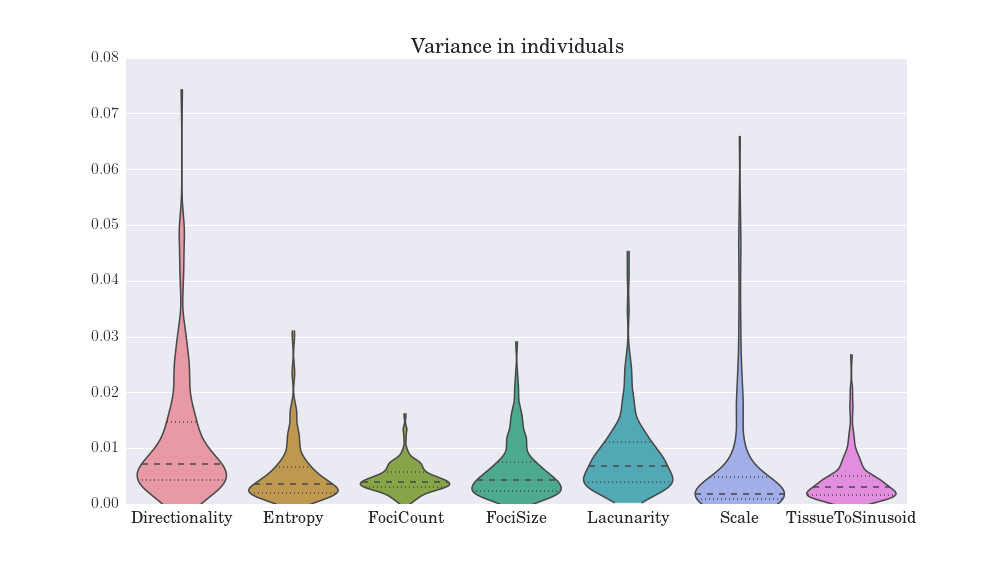
\includegraphics{figures/intra.png}
\caption{image}
\end{figure}

    \begin{figure}[htbp]
\centering
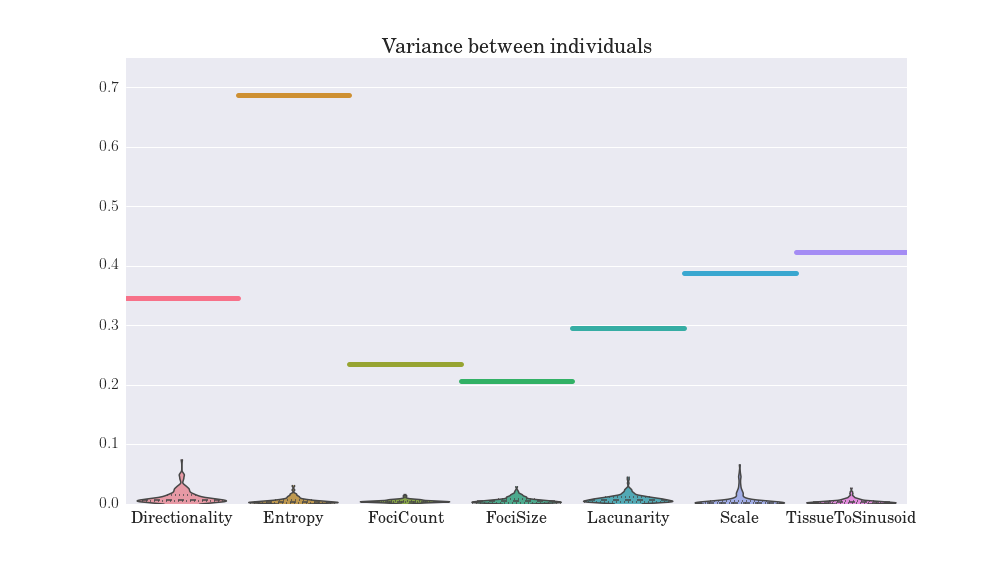
\includegraphics{figures/inter2.png}
\caption{image}
\end{figure}


    \subsection{Exploratory Analysis}



    \subsubsection{by individual}


    \begin{Verbatim}[commandchars=\\\{\}]
{\color{incolor}In [{\color{incolor}29}]:} \PY{n}{portal\PYZus{}inflammation}
\end{Verbatim}

            \begin{Verbatim}[commandchars=\\\{\}]
{\color{outcolor}Out[{\color{outcolor}29}]:} <class 'statsmodels.iolib.summary.Summary'>
         """
                                      GLS Regression Results                            
         ===============================================================================
         Dep. Variable:     Portal\_inflammation   R-squared:                       0.280
         Model:                             GLS   Adj. R-squared:                  0.273
         Method:                  Least Squares   F-statistic:                     37.34
         Date:                 Tue, 28 Oct 2014   Prob (F-statistic):           2.12e-08
         Time:                         23:40:10   Log-Likelihood:                 14.996
         No. Observations:                   98   AIC:                            -25.99
         Df Residuals:                       96   BIC:                            -20.82
         Df Model:                            1                                         
         Covariance Type:             nonrobust                                         
         ==============================================================================
                          coef    std err          t      P>|t|      [95.0\% Conf. Int.]
         ------------------------------------------------------------------------------
         FociSize       0.5627      0.092      6.111      0.000         0.380     0.746
         Intercept      0.3368      0.043      7.855      0.000         0.252     0.422
         ==============================================================================
         
         Warnings:
         [1] Standard Errors assume that the covariance matrix of the errors is correctly specified.
         """
\end{Verbatim}
        
    \begin{figure}[htbp]
\centering
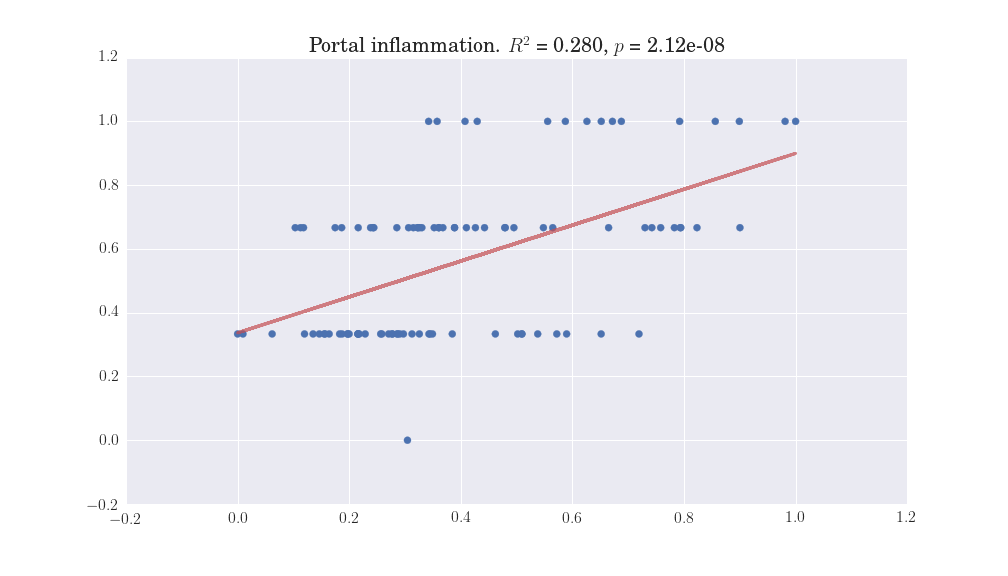
\includegraphics{figures/portal_inflammation.png}
\caption{image}
\end{figure}

    \begin{Verbatim}[commandchars=\\\{\}]
{\color{incolor}In [{\color{incolor}31}]:} \PY{n}{hyperplasia}
\end{Verbatim}

            \begin{Verbatim}[commandchars=\\\{\}]
{\color{outcolor}Out[{\color{outcolor}31}]:} <class 'statsmodels.iolib.summary.Summary'>
         """
                                     GLS Regression Results                            
         ==============================================================================
         Dep. Variable:         BD\_hyperplasia   R-squared:                       0.306
         Model:                            GLS   Adj. R-squared:                  0.284
         Method:                 Least Squares   F-statistic:                     13.83
         Date:                Tue, 28 Oct 2014   Prob (F-statistic):           1.52e-07
         Time:                        23:40:10   Log-Likelihood:                -3.9632
         No. Observations:                  98   AIC:                             15.93
         Df Residuals:                      94   BIC:                             26.27
         Df Model:                           3                                         
         Covariance Type:            nonrobust                                         
         ==================================================================================
                              coef    std err          t      P>|t|      [95.0\% Conf. Int.]
         ----------------------------------------------------------------------------------
         FociSize           0.6698      0.113      5.902      0.000         0.444     0.895
         Scale              0.5811      0.243      2.394      0.019         0.099     1.063
         Directionality    -0.4419      0.190     -2.330      0.022        -0.819    -0.065
         Intercept         -0.0504      0.079     -0.642      0.523        -0.206     0.105
         ==================================================================================
         
         Warnings:
         [1] Standard Errors assume that the covariance matrix of the errors is correctly specified.
         """
\end{Verbatim}
        
    \begin{figure}[htbp]
\centering
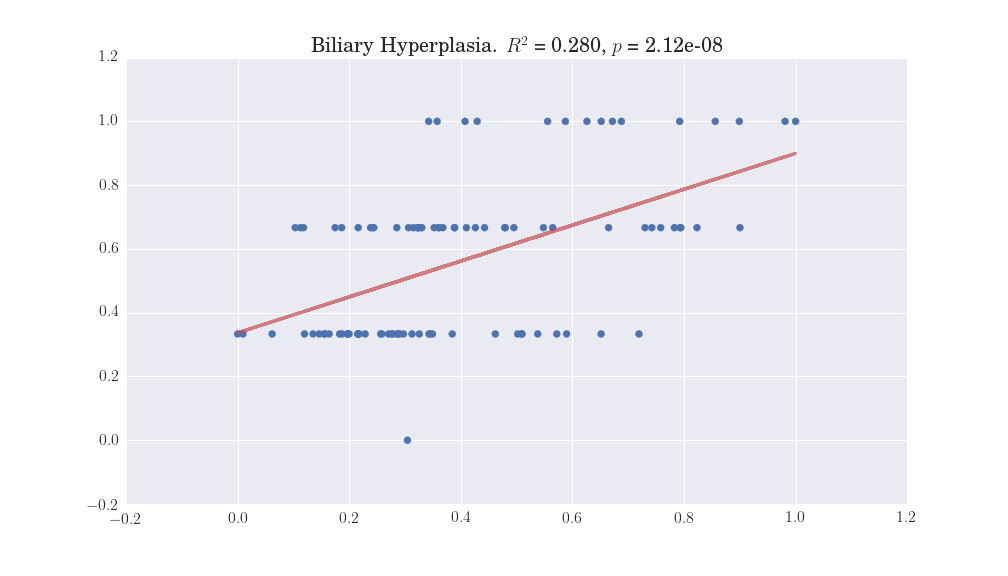
\includegraphics{figures/hyperplasia.png}
\caption{image}
\end{figure}

    \begin{Verbatim}[commandchars=\\\{\}]
{\color{incolor}In [{\color{incolor}15}]:} \PY{n}{pca}
\end{Verbatim}

            \begin{Verbatim}[commandchars=\\\{\}]
{\color{outcolor}Out[{\color{outcolor}15}]:} <class 'statsmodels.iolib.summary.Summary'>
         """
                                     GLS Regression Results                            
         ==============================================================================
         Dep. Variable:                      y   R-squared:                       0.075
         Model:                            GLS   Adj. R-squared:                  0.065
         Method:                 Least Squares   F-statistic:                     7.723
         Date:                Wed, 29 Oct 2014   Prob (F-statistic):            0.00657
         Time:                        14:38:47   Log-Likelihood:                -70.082
         No. Observations:                  97   AIC:                             144.2
         Df Residuals:                      95   BIC:                             149.3
         Df Model:                           1                                         
         Covariance Type:            nonrobust                                         
         ==============================================================================
                          coef    std err          t      P>|t|      [95.0\% Conf. Int.]
         ------------------------------------------------------------------------------
         const      -2.949e-17      0.051  -5.77e-16      1.000        -0.102     0.102
         x1             0.3865      0.139      2.779      0.007         0.110     0.663
         ==============================================================================
         
         Warnings:
         [1] Standard Errors assume that the covariance matrix of the errors is correctly specified.
         """
\end{Verbatim}
        
    \begin{figure}[htbp]
\centering
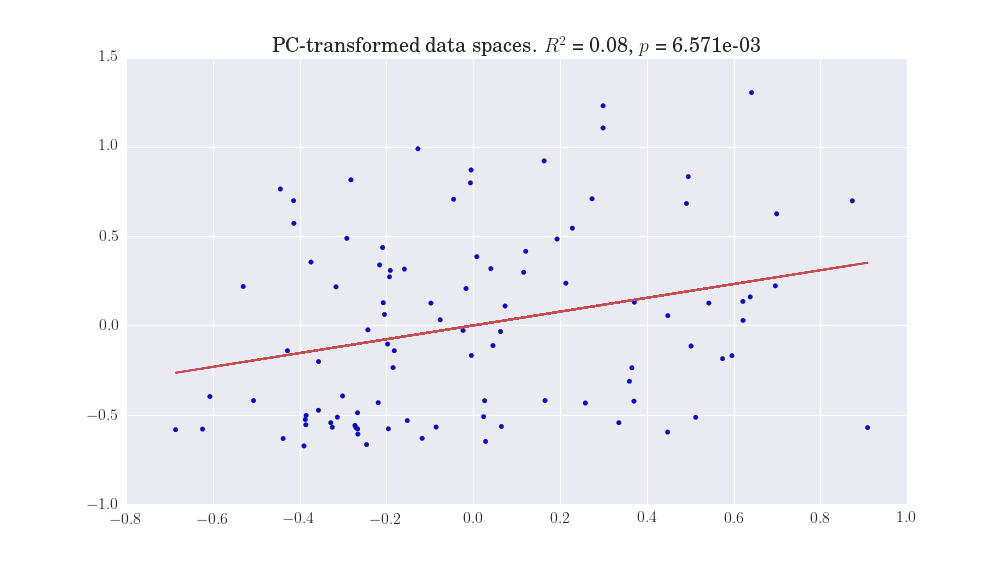
\includegraphics{figures/pca.png}
\caption{image}
\end{figure}


    \subsection{Exploratory Analysis}



    \subsubsection{by age class}


    \begin{Verbatim}[commandchars=\\\{\}]
{\color{incolor}In [{\color{incolor}6}]:} \PY{n}{fibrosis}
\end{Verbatim}

            \begin{Verbatim}[commandchars=\\\{\}]
{\color{outcolor}Out[{\color{outcolor}6}]:} <class 'statsmodels.iolib.summary.Summary'>
        """
                                    GLS Regression Results                            
        ==============================================================================
        Dep. Variable:               Fibrosis   R-squared:                       0.800
        Model:                            GLS   Adj. R-squared:                  0.778
        Method:                 Least Squares   F-statistic:                     36.07
        Date:                Wed, 29 Oct 2014   Prob (F-statistic):           0.000201
        Time:                        11:13:48   Log-Likelihood:                 7.8003
        No. Observations:                  11   AIC:                            -11.60
        Df Residuals:                       9   BIC:                            -10.80
        Df Model:                           1                                         
        Covariance Type:            nonrobust                                         
        ================================================================================
                           coef    std err          t      P>|t|      [95.0\% Conf. Int.]
        --------------------------------------------------------------------------------
        Inflammation     1.0159      0.169      6.006      0.000         0.633     1.399
        Intercept       -0.0105      0.083     -0.126      0.902        -0.198     0.177
        ================================================================================
        
        Warnings:
        [1] Standard Errors assume that the covariance matrix of the errors is correctly specified.
        """
\end{Verbatim}
        
    \begin{figure}[htbp]
\centering
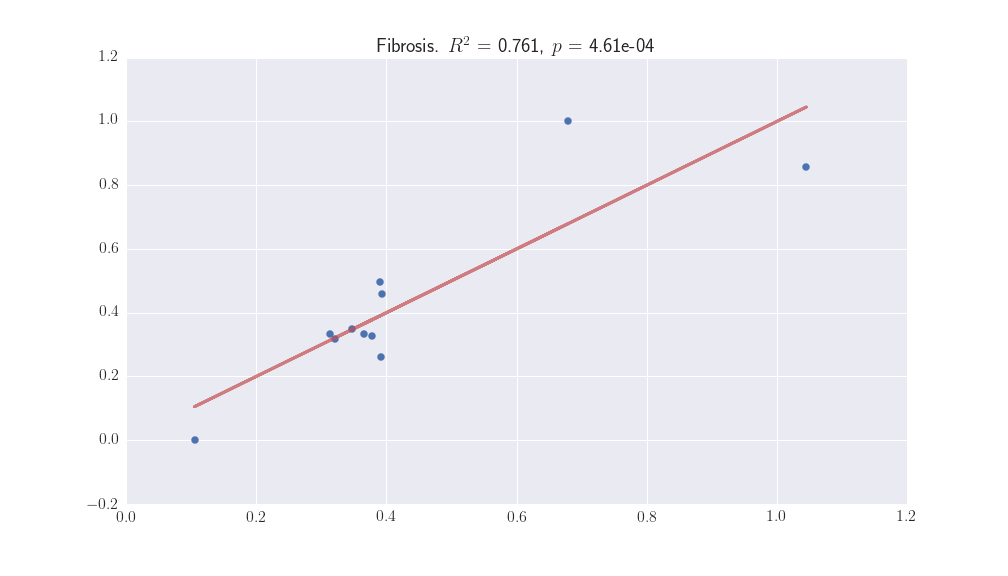
\includegraphics{figures/fibrosis.png}
\caption{image}
\end{figure}

    \begin{Verbatim}[commandchars=\\\{\}]
{\color{incolor}In [{\color{incolor}7}]:} \PY{n}{lobular\PYZus{}collapse}
\end{Verbatim}

            \begin{Verbatim}[commandchars=\\\{\}]
{\color{outcolor}Out[{\color{outcolor}7}]:} <class 'statsmodels.iolib.summary.Summary'>
        """
                                    GLS Regression Results                            
        ==============================================================================
        Dep. Variable:       Lobular\_collapse   R-squared:                       0.586
        Model:                            GLS   Adj. R-squared:                  0.540
        Method:                 Least Squares   F-statistic:                     12.73
        Date:                Wed, 29 Oct 2014   Prob (F-statistic):            0.00605
        Time:                        11:13:48   Log-Likelihood:                 2.2626
        No. Observations:                  11   AIC:                           -0.5252
        Df Residuals:                       9   BIC:                            0.2706
        Df Model:                           1                                         
        Covariance Type:            nonrobust                                         
        ==============================================================================
                         coef    std err          t      P>|t|      [95.0\% Conf. Int.]
        ------------------------------------------------------------------------------
        FociSize       1.1379      0.319      3.567      0.006         0.416     1.860
        Intercept      0.0460      0.159      0.289      0.779        -0.314     0.406
        ==============================================================================
        
        Warnings:
        [1] Standard Errors assume that the covariance matrix of the errors is correctly specified.
        """
\end{Verbatim}
        
    \begin{figure}[htbp]
\centering
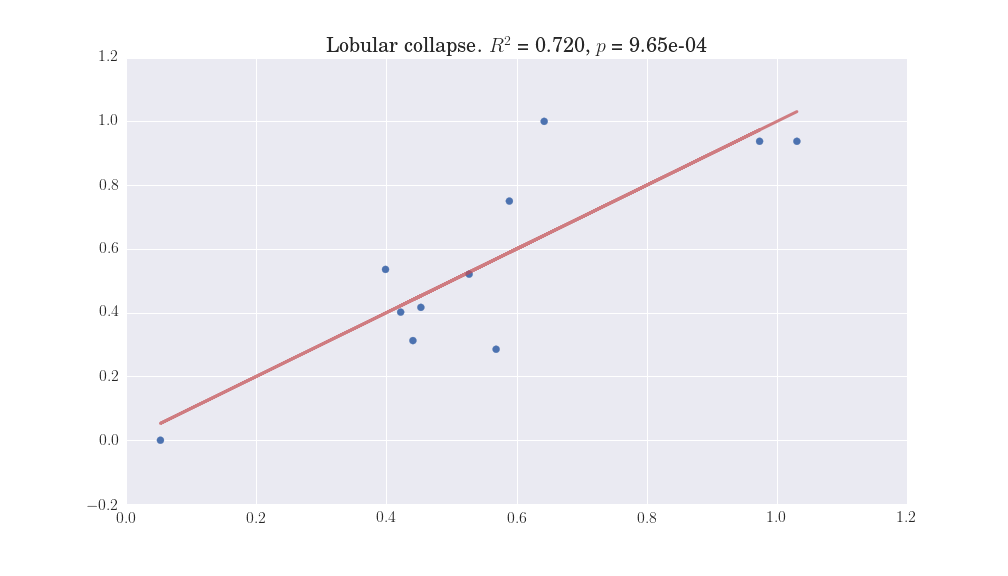
\includegraphics{figures/lobular_collapse.png}
\caption{image}
\end{figure}

    \begin{Verbatim}[commandchars=\\\{\}]
{\color{incolor}In [{\color{incolor}8}]:} \PY{n}{interface\PYZus{}hepatitis}
\end{Verbatim}

            \begin{Verbatim}[commandchars=\\\{\}]
{\color{outcolor}Out[{\color{outcolor}8}]:} <class 'statsmodels.iolib.summary.Summary'>
        """
                                     GLS Regression Results                            
        ===============================================================================
        Dep. Variable:     Interface\_hepatitis   R-squared:                       0.659
        Model:                             GLS   Adj. R-squared:                  0.621
        Method:                  Least Squares   F-statistic:                     17.38
        Date:                 Wed, 29 Oct 2014   Prob (F-statistic):            0.00242
        Time:                         11:13:48   Log-Likelihood:                 2.3063
        No. Observations:                   11   AIC:                           -0.6126
        Df Residuals:                        9   BIC:                            0.1832
        Df Model:                            1                                         
        Covariance Type:             nonrobust                                         
        ==============================================================================
                         coef    std err          t      P>|t|      [95.0\% Conf. Int.]
        ------------------------------------------------------------------------------
        Lacunarity    -1.0224      0.245     -4.168      0.002        -1.577    -0.468
        Intercept      0.9504      0.143      6.669      0.000         0.628     1.273
        ==============================================================================
        
        Warnings:
        [1] Standard Errors assume that the covariance matrix of the errors is correctly specified.
        """
\end{Verbatim}
        
    \begin{figure}[htbp]
\centering
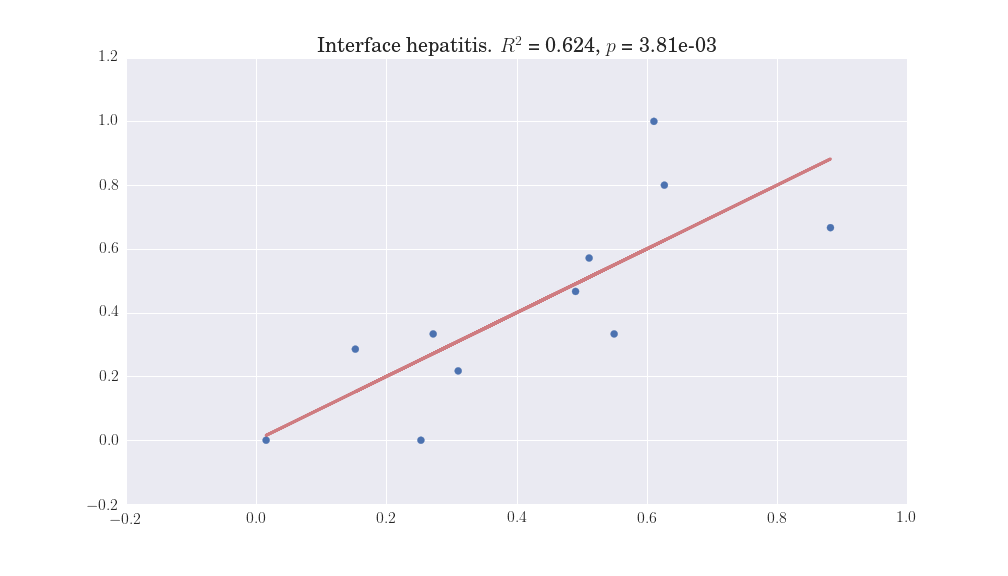
\includegraphics{figures/interface_hepatitis.png}
\caption{image}
\end{figure}


    \subsection{Exploratory analysis}



    \subsubsection{with a random effect on age at death}


    \begin{longtable}[c]{@{}lcl@{}}
\toprule\addlinespace
Dependent variable & Models AIC \textless{} 2 + AICmin & Primary
explanatory variables ( ordered )
\\\addlinespace
\midrule\endhead
Ishak score & 7 & entropy, tissue-to-sinusoid, focus count, focus size
\\\addlinespace
Lobular collapse & 5 & entropy, lacunarity, tissue-to-sinusoid, focus
count
\\\addlinespace
Confluent necrosis & 1 & entropy
\\\addlinespace
Interface hepatitis & 2 & entropy, tissue-to-sinusoid
\\\addlinespace
Portal inflammation & 4 & entropy, focus size, lacunarity, focus count,
scale, directionality
\\\addlinespace
Fibrosis & 2 & entropy, lacunarity, tissue-to-sinusoid
\\\addlinespace
Biliary hyperplasia & 1 & focus size
\\\addlinespace
Necrosis, apoptosis, random inflammation & 2 & entropy, lacunarity
\\\addlinespace
\bottomrule
\end{longtable}


    \paragraph{Measures we like}


    \begin{itemize}
\itemsep1pt\parskip0pt\parsep0pt
\item
  entropy consistently explains histological measures when controlled
  for age
\item
  also important : tissue to sinusoid ratio, focus count and size,
  lacunarity
\end{itemize}


    \subsection{Future directions}



    \subsubsection{Further exploration of the dataset}


    \begin{itemize}
\item
  145 sheep ( 89 females )
\item
  11 age classes
\item
\end{itemize}

    \begin{itemize}
\itemsep1pt\parskip0pt\parsep0pt
\item
  4460 entries across 27 variables
\item
  3330 with full image and histological information
\item
  1196 for which \textbf{complete} information is available
\end{itemize}


    \subsubsection{Narrow-field images}


    \begin{itemize}
\itemsep1pt\parskip0pt\parsep0pt
\item
  12536 images
\item
  spatial distribution of nuclei
\end{itemize}

    \begin{figure}[htbp]
\centering
\includegraphics{figures/10.jpg}
\caption{image}
\end{figure}

    \begin{figure}[htbp]
\centering
\includegraphics{figures/Processed2.jpg}
\caption{image}
\end{figure}

    \begin{figure}[htbp]
\centering
\includegraphics{figures/Segmented.jpg}
\caption{image}
\end{figure}

    


    % Add a bibliography block to the postdoc
    
    
    
    \end{document}
